% !TeX program = xelatex
% !TeX encoding = UTF-8
% 忠实格式版：保留原样本中的红色说明、手工目录及原编号。
\documentclass[12pt,a4paper]{article}
\usepackage{word-layout}
\begin{document}
\hypersetup{pageanchor=false}
\pagestyle{wordcover}
% UTF-8。保留原文文字、颜色、字号、缩进和空段落；最后一项参数是可编辑文本。

% 原文段落 000；
\begin{WordParagraph}{center}{12}{\WordAutoLine{12}{1.25}}{0}{0}{0}{0}{0}
\WordAutoSpaceOn
\WordEmpty
\end{WordParagraph}

% 原文段落 001；
\begin{WordParagraph}{center}{12}{\WordAutoLine{12}{1.25}}{0}{0}{0}{0}{0}
\WordAutoSpaceOn

\includegraphics[width=7.3554cm,height=1.2435cm]{assets/hust-logo.png}
\end{WordParagraph}

% 原文段落 002；
\begin{WordParagraph}{both}{12}{\WordAutoLine{12}{1.25}}{0}{0}{0}{0}{0}
\WordAutoSpaceOn
\WordEmpty
\end{WordParagraph}

% 原文段落 003；
\begin{WordParagraph}{both}{12}{\WordAutoLine{12}{1.25}}{0}{0}{0}{0}{0}
\WordAutoSpaceOn
\WordEmpty
\end{WordParagraph}

% 原文段落 004；《软件工程》项目报告
\begin{WordParagraph}{center}{36}{\WordAutoLine{36}{1.25}}{0}{0}{0}{0}{0}
\WordAutoSpaceOn
\WordRun{Fang}{Fang}{36}{1}{0}{000000}{0}{《软件工程》项目报告}
\end{WordParagraph}

% 原文段落 005；
\begin{WordParagraph}{both}{12}{\WordAutoLine{12}{1.25}}{0}{0}{0}{0}{0}
\WordAutoSpaceOn
\WordEmpty
\end{WordParagraph}

% 原文段落 006；
\begin{WordParagraph}{both}{12}{\WordAutoLine{12}{1.25}}{0}{0}{0}{0}{0}
\WordAutoSpaceOn
\WordEmpty
\end{WordParagraph}

% 原文段落 007；
\begin{WordParagraph}{both}{18}{\WordAutoLine{18}{1.25}}{0}{0}{0}{0}{0}
\WordAutoSpaceOn
\WordEmpty
\end{WordParagraph}

% 原文段落 008；题目：                             
\begin{WordParagraph}{both}{18}{\WordAutoLine{18}{1.25}}{0}{0}{34.9}{0}{0}
\WordAutoSpaceOn
\WordRun{Hei}{Hei}{18}{1}{0}{000000}{0}{题目}%
\WordRun{Times}{Song}{18}{1}{0}{000000}{0}{：}%
\WordRun{Times}{Song}{18}{1}{0}{000000}{1}{\WordSpace{29}}
\end{WordParagraph}

% 原文段落 009；
\begin{WordParagraph}{both}{12}{\WordAutoLine{12}{1.25}}{0}{0}{0}{0}{0}
\WordAutoSpaceOn
\WordEmpty
\end{WordParagraph}

% 原文段落 010；
\begin{WordParagraph}{both}{12}{\WordAutoLine{12}{1.25}}{0}{0}{0}{0}{0}
\WordAutoSpaceOn
\WordEmpty
\end{WordParagraph}

% 原文段落 011；
\begin{WordParagraph}{both}{12}{\WordAutoLine{12}{1.25}}{0}{0}{0}{0}{0}
\WordAutoSpaceOn
\WordEmpty
\end{WordParagraph}

% 原文段落 012；
\begin{WordParagraph}{both}{12}{\WordAutoLine{12}{1.25}}{0}{0}{0}{0}{0}
\WordAutoSpaceOn
\WordEmpty
\end{WordParagraph}

% 原文段落 013；课程名称：      软件工程         
\begin{WordParagraph}{both}{14}{\WordAutoLine{14}{1.25}}{0}{0}{90.25}{0}{0}
\WordAutoSpaceOn
\WordRun{Times}{Song}{14}{1}{0}{000000}{0}{课程名称：}%
\WordRun{Times}{Song}{14}{1}{0}{000000}{1}{\WordSpace{6}软件工程\WordSpace{9}}
\end{WordParagraph}

% 原文段落 014；专业班级：                       
\begin{WordParagraph}{both}{14}{\WordAutoLine{14}{1.25}}{0}{0}{90.25}{0}{0}
\WordAutoSpaceOn
\WordRun{Times}{Song}{14}{1}{0}{000000}{0}{专业班级：}%
\WordRun{Times}{Song}{14}{1}{0}{000000}{1}{\WordSpace{23}}
\end{WordParagraph}

% 原文段落 015；            组    号：按照检查表中的班级序号，例如： CS2404 ①           
\begin{WordParagraph}{center}{14}{\WordAutoLine{14}{1.25}}{0}{0}{0}{0}{0}
\WordAutoSpaceOn
\WordRun{Times}{Song}{14}{1}{0}{000000}{0}{\WordSpace{12}组\WordSpace{4}号：}%
\WordRun{Times}{Song}{12}{1}{0}{C00000}{1}{按照检查表中的班级序号，例如：\WordSpace{1}}%
\WordRun{Times}{Song}{12}{0}{0}{C00000}{0}{CS2404}%
\WordRun{Times}{Song}{14}{1}{0}{C00000}{1}{\WordSpace{1}}%
\WordRun{Times}{Song}{12}{0}{0}{C00000}{0}{①}%
\WordRun{Times}{Song}{14}{1}{0}{000000}{1}{\WordSpace{11}}
\end{WordParagraph}

% 原文段落 016；同组成员： 学号：                
\begin{WordParagraph}{both}{14}{\WordAutoLine{14}{1.25}}{0}{0}{90.25}{0}{0}
\WordAutoSpaceOn
\WordRun{Times}{Song}{14}{1}{0}{000000}{0}{同组成员：}%
\WordRun{Times}{Song}{14}{1}{0}{000000}{1}{\WordSpace{1}学号：\WordSpace{16}}
\end{WordParagraph}

% 原文段落 017； 姓名：                
\begin{WordParagraph}{both}{14}{\WordAutoLine{14}{1.25}}{0}{0}{160.5}{0}{0}
\WordAutoSpaceOn
\WordRun{Times}{Song}{14}{1}{0}{000000}{1}{\WordSpace{1}姓名：\WordSpace{16}}
\end{WordParagraph}

% 原文段落 018； 学号：                
\begin{WordParagraph}{both}{14}{\WordAutoLine{14}{1.25}}{0}{0}{160.5}{0}{0}
\WordAutoSpaceOn
\WordRun{Times}{Song}{14}{1}{0}{000000}{1}{\WordSpace{1}学号：\WordSpace{16}}
\end{WordParagraph}

% 原文段落 019； 姓名：                
\begin{WordParagraph}{both}{14}{\WordAutoLine{14}{1.25}}{0}{0}{160.5}{0}{0}
\WordAutoSpaceOn
\WordRun{Times}{Song}{14}{1}{0}{000000}{1}{\WordSpace{1}姓名：\WordSpace{16}}
\end{WordParagraph}

% 原文段落 020； 学号：                
\begin{WordParagraph}{both}{14}{\WordAutoLine{14}{1.25}}{0}{0}{160.5}{0}{0}
\WordAutoSpaceOn
\WordRun{Times}{Song}{14}{1}{0}{000000}{1}{\WordSpace{1}学号：\WordSpace{16}}
\end{WordParagraph}

% 原文段落 021； 姓名：                
\begin{WordParagraph}{both}{14}{\WordAutoLine{14}{1.25}}{0}{0}{160.5}{0}{0}
\WordAutoSpaceOn
\WordRun{Times}{Song}{14}{1}{0}{000000}{1}{\WordSpace{1}姓名：\WordSpace{16}}
\end{WordParagraph}

% 原文段落 022； 学号：                
\begin{WordParagraph}{both}{14}{\WordAutoLine{14}{1.25}}{0}{0}{160.5}{0}{0}
\WordAutoSpaceOn
\WordRun{Times}{Song}{14}{1}{0}{000000}{1}{\WordSpace{1}学号：\WordSpace{16}}
\end{WordParagraph}

% 原文段落 023； 姓名：                
\begin{WordParagraph}{both}{14}{\WordAutoLine{14}{1.25}}{0}{0}{160.5}{0}{0}
\WordAutoSpaceOn
\WordRun{Times}{Song}{14}{1}{0}{000000}{1}{\WordSpace{1}姓名：\WordSpace{16}}
\end{WordParagraph}

% 原文段落 024；指导教师：                       
\begin{WordParagraph}{both}{14}{\WordAutoLine{14}{1.25}}{0}{0}{90.25}{0}{0}
\WordAutoSpaceOn
\WordRun{Times}{Song}{14}{1}{0}{000000}{0}{指导教师：}%
\WordRun{Times}{Song}{14}{1}{0}{000000}{1}{\WordSpace{23}}
\end{WordParagraph}

% 原文段落 025；报告日期：                       
\begin{WordParagraph}{both}{14}{\WordAutoLine{14}{1.25}}{0}{0}{90.25}{0}{0}
\WordAutoSpaceOn
\WordRun{Times}{Song}{14}{1}{0}{000000}{0}{报告日期：}%
\WordRun{Times}{Song}{14}{1}{0}{000000}{1}{\WordSpace{23}}
\end{WordParagraph}

% 原文段落 026；
\begin{WordParagraph}{both}{12}{\WordAutoLine{12}{1.25}}{0}{0}{0}{0}{0}
\WordAutoSpaceOn
\WordEmpty
\end{WordParagraph}

% 原文段落 027；
\begin{WordParagraph}{both}{12}{\WordAutoLine{12}{1.25}}{0}{0}{0}{0}{0}
\WordAutoSpaceOn
\WordEmpty
\end{WordParagraph}

% 原文段落 028；
\begin{WordParagraph}{both}{12}{\WordAutoLine{12}{1.25}}{0}{0}{0}{0}{0}
\WordAutoSpaceOn
\WordEmpty
\end{WordParagraph}

% 原文段落 029；计算机科学与技术学院
\begin{WordParagraph}{center}{14}{\WordAutoLine{14}{1.25}}{0}{0}{0}{0}{0}
\WordAutoSpaceOn
\WordRun{Times}{Song}{14}{1}{0}{000000}{0}{计算机科学与技术学院}
\end{WordParagraph}

\clearpage
\hypersetup{pageanchor=true}
\pagenumbering{Roman}
\pagestyle{wordfront}
% UTF-8。保留原文文字、颜色、字号、缩进和空段落；最后一项参数是可编辑文本。

% 原文段落 030；
\begin{WordParagraph}{center}{14}{\WordAutoLine{14}{1.25}}{0}{0}{0}{0}{0}
\WordAutoSpaceOn
\WordEmpty
\end{WordParagraph}

% 原文段落 031；任 务 书（黑体小2号加粗居中）
\begin{WordParagraph}{center}{18}{\WordAutoLine{18}{1}}{0}{0}{0}{0}{0}
\WordAutoSpaceOn
\WordRun{Times}{Hei}{18}{1}{0}{000000}{0}{任\WordSpace{1}务\WordSpace{1}书}%
\WordRun{Kai}{Kai}{12}{0}{0}{FF0000}{0}{（黑体小2号加粗居中）}
\end{WordParagraph}

% 原文段落 032；一 总体要求（黑体4号加粗,字母、阿拉伯数字为Time New Roman4号加粗）
\begin{WordParagraph}{both}{14}{\WordAutoLine{14}{1.5}}{0}{0}{0}{0}{0}
\WordAutoSpaceOn
\WordRun{Hei}{Hei}{14}{1}{0}{000000}{0}{一\WordSpace{1}总体要求}%
\WordRun{Kai}{Kai}{12}{0}{0}{FF0000}{0}{（黑体4号加粗,字母、阿拉伯数字为Time\WordSpace{1}New\WordSpace{1}Roman4号加粗）}
\end{WordParagraph}

% 原文段落 033；1. 综合运用软件工程的思想，协同完成一个软件项目的开发，掌软件工程相关的技术和方法；
\begin{WordParagraph}{both}{12}{\WordAutoLine{12}{1.5}}{12}{0}{-12}{0}{0}
\WordAutoSpaceOn
\WordRun{Times}{Song}{12}{0}{0}{000000}{0}{1.\WordSpace{1}综合运用软件工程的思想，协同完成一个软件项目的开发，掌软件工程相关的技术和方法；}
\end{WordParagraph}

% 原文段落 034；2. 组成小组进行选题，通过调研完成项目的需求分析，并详细说明小组成员的分工、项目的时间管理等方面。
\begin{WordParagraph}{both}{12}{\WordAutoLine{12}{1.5}}{12}{0}{-12}{0}{0}
\WordAutoSpaceOn
\WordRun{Times}{Song}{12}{0}{0}{000000}{0}{2.\WordSpace{1}组成小组进行选题，通过调研完成项目的需求分析，并详细说明小组成员的分工、项目的时间管理等方面。}
\end{WordParagraph}

% 原文段落 035；3. 根据需求分析进行总体设计、详细设计、编码与测试等。
\begin{WordParagraph}{both}{12}{\WordAutoLine{12}{1.5}}{0}{0}{0}{0}{0}
\WordAutoSpaceOn
\WordRun{Times}{Song}{12}{0}{0}{000000}{0}{3.\WordSpace{1}根据需求分析进行总体设计、详细设计、编码与测试等。}
\end{WordParagraph}

% 原文段落 036；二 基本内容（黑体4号加粗,字母、阿拉伯数字为Time New Roman4号加粗）
\begin{WordParagraph}{both}{14}{\WordAutoLine{14}{1.5}}{0}{0}{0}{0}{0}
\WordAutoSpaceOn
\WordRun{Hei}{Hei}{14}{1}{0}{000000}{0}{二\WordSpace{1}基本内容}%
\WordRun{Kai}{Kai}{12}{0}{0}{FF0000}{0}{（黑体4号加粗,字母、阿拉伯数字为Time\WordSpace{1}New\WordSpace{1}Roman4号加粗）}
\end{WordParagraph}

% 原文段落 037；根据给出的题目任选一题，自行组队，设计与开发中软件过程必须包括：
\begin{WordParagraph}{both}{12}{\WordAutoLine{12}{1.5}}{0}{0}{0}{0}{0}
\WordAutoSpaceOn
\WordRun{Song}{Song}{12}{0}{0}{000000}{0}{根据给出的题目任选一题，自行组队，设计与开发中软件过程必须包括：}
\end{WordParagraph}

% 原文段落 038；1. 问题概述、需求分析：正确使用相关工具和方法说明所开发软件的问题定义和需求分析，比如NABCD模型，Microsoft Visio，StarUML等工具 (20%)；
\begin{WordParagraph}{both}{12}{\WordAutoLine{12}{1.5}}{12.05}{0}{-12.05}{0}{0}
\WordAutoSpaceOn
\WordRun{Times}{Song}{12}{1}{0}{000000}{0}{1.\WordSpace{1}问题概述、需求分析：}%
\WordRun{Times}{Song}{12}{0}{0}{000000}{0}{正确使用相关工具和方法说明所开发软件的问题定义和需求分析，比如NABCD模型，Microsoft\WordSpace{1}Visio，StarUML等工具\WordSpace{1}(20\%)；}
\end{WordParagraph}

% 原文段落 039；2. 原型系统设计、概要设计、详细设计：主要说明所开发软件的架构、数据结构及主要算法设计，比如墨刀等工具（35%）；
\begin{WordParagraph}{both}{12}{\WordAutoLine{12}{1.5}}{12.05}{0}{-12.05}{0}{0}
\WordAutoSpaceOn
\WordRun{Times}{Song}{12}{1}{0}{000000}{0}{2.\WordSpace{1}原型系统设计、概要设计、详细设计}%
\WordRun{Times}{Song}{12}{0}{0}{000000}{0}{：主要说明所开发软件的架构、数据结构及主要算法设计，比如墨刀等工具（35\%）；}
\end{WordParagraph}

% 原文段落 040；3. 编码与测试：编码规范，运用码云等平台进行版本管理，设计测试计划和测试用例（30%）；
\begin{WordParagraph}{both}{12}{\WordAutoLine{12}{1.5}}{12.05}{0}{-12.05}{0}{0}
\WordAutoSpaceOn
\WordRun{Times}{Song}{12}{1}{0}{000000}{0}{3.\WordSpace{1}编码与测试}%
\WordRun{Times}{Song}{12}{0}{0}{000000}{0}{：编码规范，运用码云等平台进行版本管理，设计测试计划和测试用例（30\%）；}
\end{WordParagraph}

% 原文段落 041；4．功能创新：与众不同、特别吸引用户的创新（10%）；
\begin{WordParagraph}{both}{12}{\WordAutoLine{12}{1.5}}{12.05}{0}{-12.05}{0}{0}
\WordAutoSpaceOn
\WordRun{Times}{Song}{12}{1}{0}{000000}{0}{4．功能创新}%
\WordRun{Times}{Song}{12}{0}{0}{000000}{0}{：与众不同、特别吸引用户的创新（10\%）；}
\end{WordParagraph}

% 原文段落 042；5. 用户反馈：包括用户的使用记录，照片，视频等（5%）。
\begin{WordParagraph}{both}{12}{\WordAutoLine{12}{1.5}}{12.05}{0}{-12.05}{0}{0}
\WordAutoSpaceOn
\WordRun{Times}{Song}{12}{1}{0}{000000}{0}{5.\WordSpace{1}用户反馈}%
\WordRun{Times}{Song}{12}{0}{0}{000000}{0}{：包括用户的使用记录，照片，视频等（5\%）。}
\end{WordParagraph}

% 原文段落 043；
\begin{WordParagraph}{both}{12}{\WordAutoLine{12}{1.5}}{12}{0}{-12}{0}{0}
\WordAutoSpaceOn
\WordEmpty
\end{WordParagraph}

% 原文段落 044；
\begin{WordParagraph}{both}{12}{\WordAutoLine{12}{1.5}}{12}{0}{-12}{0}{0}
\WordAutoSpaceOn
\WordEmpty
\end{WordParagraph}

% 原文段落 045；
\begin{WordParagraph}{both}{12}{\WordAutoLine{12}{1.5}}{12}{0}{-12}{0}{0}
\WordAutoSpaceOn
\WordEmpty
\end{WordParagraph}

% 原文段落 046；
\begin{WordParagraph}{both}{12}{\WordAutoLine{12}{1.5}}{12}{0}{-12}{0}{0}
\WordAutoSpaceOn
\WordEmpty
\end{WordParagraph}

% 原文段落 047；
\begin{WordParagraph}{both}{12}{\WordAutoLine{12}{1.5}}{0}{0}{0}{0}{0}
\WordAutoSpaceOn
\WordEmpty
\end{WordParagraph}

% 原文段落 048；
\begin{WordParagraph}{both}{12}{\WordAutoLine{12}{1.5}}{0}{0}{0}{0}{0}
\WordAutoSpaceOn
\WordEmpty
\end{WordParagraph}

% 原文段落 049；
\begin{WordParagraph}{both}{12}{\WordAutoLine{12}{1.5}}{0}{0}{0}{0}{0}
\WordAutoSpaceOn
\WordEmpty
\end{WordParagraph}

% 原文段落 050；
\begin{WordParagraph}{both}{12}{\WordAutoLine{12}{1.5}}{0}{0}{0}{0}{0}
\WordAutoSpaceOn
\WordEmpty
\end{WordParagraph}

% 原文段落 051；
\begin{WordParagraph}{both}{12}{\WordAutoLine{12}{1.5}}{0}{0}{0}{0}{0}
\WordAutoSpaceOn
\WordEmpty
\end{WordParagraph}

% 原文段落 052；
\begin{WordParagraph}{both}{12}{\WordAutoLine{12}{1.5}}{0}{0}{0}{0}{0}
\WordAutoSpaceOn
\WordEmpty
\end{WordParagraph}

% 原文段落 053；
\begin{WordParagraph}{both}{12}{\WordAutoLine{12}{1.5}}{0}{0}{0}{0}{0}
\WordAutoSpaceOn
\WordEmpty
\end{WordParagraph}

% 原样本通过空段落把目录移到下一页；此处固定这一版面边界。
\clearpage
% UTF-8。保留原文文字、颜色、字号、缩进和空段落；最后一项参数是可编辑文本。

% 原文段落 054；目   录（黑体小2号加粗居中）
\begin{WordParagraph}{center}{18}{\WordAutoLine{18}{1.25}}{20.5}{137.75}{49.5}{7.8}{7.8}
\WordAutoSpaceOn
\WordRun{Times}{Hei}{18}{1}{0}{000000}{0}{目\WordSpace{3}录}%
\WordRun{Kai}{Kai}{12}{0}{0}{FF0000}{0}{（黑体小2号加粗居中）}
\end{WordParagraph}

% 原文段落 055；任务书 | I
\begin{WordParagraph}{both}{12}{\WordAutoLine{12}{1.5}}{0}{0}{0}{0}{0}
\WordAutoSpaceOn
\WordTOCLine{\WordRun{Song}{Song}{12}{1}{0}{0000FF}{0}{任务书}}{\WordRun{Times}{Song}{12}{0}{0}{0000FF}{0}{I}}{459}{0000FF}
\end{WordParagraph}

% 原文段落 056；1问题定义 | 1
\begin{WordParagraph}{both}{12}{\WordAutoLine{12}{1.5}}{0}{0}{0}{0}{0}
\WordAutoSpaceOn
\WordTOCLine{\WordRun{Song}{Song}{12}{1}{0}{0000FF}{0}{1问题定义}}{\WordRun{Times}{Song}{12}{0}{0}{0000FF}{0}{1}}{459}{0000FF}
\end{WordParagraph}

% 原文段落 057；1.1项目背景及意义 | 1
\begin{WordParagraph}{both}{12}{\WordAutoLine{12}{1.5}}{0}{0}{0}{0}{0}
\WordAutoSpaceOn
\WordTOCLine{\WordRun{Times}{Song}{12}{0}{0}{0000FF}{0}{1.1}\WordRun{Song}{Song}{10.5}{0}{0}{000000}{0}{项目背景及意义}}{\WordRun{Times}{Song}{12}{0}{0}{000000}{0}{1}}{459}{000000}
\end{WordParagraph}

% 原文段落 058；1.2项目基本目标 | 3
\begin{WordParagraph}{both}{12}{\WordAutoLine{12}{1.5}}{0}{0}{0}{0}{0}
\WordAutoSpaceOn
\WordTOCLine{\WordRun{Times}{Song}{12}{0}{0}{0000FF}{0}{1.2}\WordRun{Song}{Song}{10.5}{0}{0}{000000}{0}{项目基本目标}}{\WordRun{Times}{Song}{12}{0}{0}{000000}{0}{3}}{459}{000000}
\end{WordParagraph}

% 原文段落 059；1.3可行性分析 | 7
\begin{WordParagraph}{both}{12}{\WordAutoLine{12}{1.5}}{0}{0}{0}{0}{0}
\WordAutoSpaceOn
\WordTOCLine{\WordRun{Times}{Song}{12}{0}{0}{0000FF}{0}{1.3}\WordRun{Song}{Song}{10.5}{0}{0}{000000}{0}{可行性分析}}{\WordRun{Times}{Song}{12}{0}{0}{000000}{0}{7}}{459}{000000}
\end{WordParagraph}

% 原文段落 060；1.4人员管理和项目进度管理 | 9
\begin{WordParagraph}{both}{12}{\WordAutoLine{12}{1.5}}{0}{0}{0}{0}{0}
\WordAutoSpaceOn
\WordTOCLine{\WordRun{Times}{Song}{12}{0}{0}{0000FF}{0}{1.4}\WordRun{Song}{Song}{10.5}{0}{0}{000000}{0}{人员}\WordRun{Song}{Song}{10.5}{0}{0}{000000}{0}{管理和项目进度管理}}{\WordRun{Times}{Song}{12}{0}{0}{000000}{0}{9}}{459}{000000}
\end{WordParagraph}

% 原文段落 061；……
\begin{WordParagraph}{center}{12}{\WordAutoLine{12}{1.5}}{0}{0}{0}{0}{0}
\WordAutoSpaceOn
\WordRun{Times}{Song}{12}{1}{0}{000000}{0}{……}
\end{WordParagraph}

% 原文段落 062；2需求分析 | 20
\begin{WordParagraph}{both}{12}{\WordAutoLine{12}{1.5}}{0}{0}{0}{0}{0}
\WordAutoSpaceOn
\WordTOCLine{\WordRun{Times}{Song}{12}{0}{0}{0000FF}{0}{2}\WordRun{Times}{Song}{12}{0}{0}{0000FF}{0}{需求分析}}{\WordRun{Times}{Song}{12}{0}{0}{0000FF}{0}{20}}{459}{0000FF}
\end{WordParagraph}

% 原文段落 063；2.1 需求分析概述 | 20
\begin{WordParagraph}{both}{12}{\WordAutoLine{12}{1.5}}{0}{0}{0}{0}{0}
\WordAutoSpaceOn
\WordTOCLine{\WordRun{Times}{Song}{12}{0}{0}{0000FF}{0}{2.1\WordSpace{1}}\WordRun{Times}{Song}{10.5}{0}{0}{000000}{0}{需求分析概述}}{\WordRun{Times}{Song}{12}{0}{0}{000000}{0}{20}}{459}{000000}
\end{WordParagraph}

% 原文段落 064；2.2 UML相关需求分析图 | 23
\begin{WordParagraph}{both}{12}{\WordAutoLine{12}{1.5}}{0}{0}{0}{0}{0}
\WordAutoSpaceOn
\WordTOCLine{\WordRun{Times}{Song}{12}{0}{0}{0000FF}{0}{2.2}\WordRun{Times}{Song}{12}{0}{0}{000000}{0}{\WordSpace{1}}\WordRun{Times}{Song}{10.5}{0}{0}{000000}{0}{UML相关需求分析图}}{\WordRun{Times}{Song}{12}{0}{0}{000000}{0}{2}\WordRun{Times}{Song}{12}{0}{0}{000000}{0}{3}}{459}{000000}
\end{WordParagraph}

% 原文段落 065；2.3原型系统设计 | 25
\begin{WordParagraph}{both}{12}{\WordAutoLine{12}{1.5}}{0}{0}{0}{0}{0}
\WordAutoSpaceOn
\WordTOCLine{\WordRun{Times}{Song}{12}{0}{0}{0000FF}{0}{2.}\WordRun{Times}{Song}{12}{0}{0}{0000FF}{0}{3}\WordRun{Song}{Song}{10.5}{0}{0}{000000}{0}{原型系统设计}}{\WordRun{Times}{Song}{12}{0}{0}{000000}{0}{25}}{459}{000000}
\end{WordParagraph}

% 原文段落 066；2.3.1  ×××××× | 30
\begin{WordParagraph}{both}{12}{\WordAutoLine{12}{1.5}}{0}{0}{0}{0}{0}
\WordAutoSpaceOn
\WordTOCLine{\WordRun{Times}{Song}{12}{0}{0}{0000FF}{0}{2}\WordRun{Times}{Song}{12}{0}{0}{0000FF}{0}{.}\WordRun{Times}{Song}{12}{0}{0}{0000FF}{0}{3.1}\WordRun{Song}{Song}{10.5}{0}{0}{000000}{0}{\WordSpace{2}}\WordRun{Song}{Song}{12}{0}{0}{0000FF}{0}{\WordHAnsi{Song}{×}\hskip0pt plus .05em\relax{}\WordHAnsi{Song}{×}\hskip0pt plus .05em\relax{}\WordHAnsi{Song}{×}\hskip0pt plus .05em\relax{}\WordHAnsi{Song}{×}\hskip0pt plus .05em\relax{}\WordHAnsi{Song}{×}\hskip0pt plus .05em\relax{}\WordHAnsi{Song}{×}\hskip0pt plus .05em\relax{}}}{\WordRun{Times}{Song}{12}{0}{0}{000000}{0}{30}}{459}{000000}
\end{WordParagraph}

% 原文段落 067；……
\begin{WordParagraph}{center}{12}{\WordAutoLine{12}{1.5}}{0}{0}{0}{0}{0}
\WordAutoSpaceOn
\WordRun{Times}{Song}{12}{1}{0}{000000}{0}{……}
\end{WordParagraph}

% 原文段落 068；3 概要设计和详细设计 | 40
\begin{WordParagraph}{both}{12}{\WordAutoLine{12}{1.5}}{0}{0}{0}{0}{0}
\WordAutoSpaceOn
\WordTOCLine{\WordRun{Times}{Song}{12}{0}{0}{0000FF}{0}{3}\WordRun{Times}{Song}{12}{0}{0}{0000FF}{0}{\WordSpace{1}概要设计和详细设计}}{\WordRun{Times}{Song}{12}{0}{0}{0000FF}{0}{4}\WordRun{Times}{Song}{12}{0}{0}{0000FF}{0}{0}}{459}{0000FF}
\end{WordParagraph}

% 原文段落 069；3.1 系统结构 | 40
\begin{WordParagraph}{both}{12}{\WordAutoLine{12}{1.5}}{0}{0}{0}{0}{0}
\WordAutoSpaceOn
\WordTOCLine{\WordRun{Times}{Song}{12}{0}{0}{0000FF}{0}{3.1\WordSpace{1}}\WordRun{Times}{Song}{10.5}{0}{0}{000000}{0}{系统}\WordRun{Times}{Song}{10.5}{0}{0}{000000}{0}{结构}}{\WordRun{Times}{Song}{12}{0}{0}{000000}{0}{4}\WordRun{Times}{Song}{12}{0}{0}{000000}{0}{0}}{459}{000000}
\end{WordParagraph}

% 原文段落 070；3.1.1功能说明 | 42
\begin{WordParagraph}{both}{12}{\WordAutoLine{12}{1.5}}{0}{0}{0}{0}{0}
\WordAutoSpaceOn
\WordTOCLine{\WordRun{Times}{Song}{12}{0}{0}{0000FF}{0}{3}\WordRun{Times}{Song}{12}{0}{0}{0000FF}{0}{.}\WordRun{Times}{Song}{12}{0}{0}{0000FF}{0}{1.1}\WordRun{Song}{Song}{10.5}{0}{0}{000000}{0}{功能说明}}{\WordRun{Times}{Song}{12}{0}{0}{000000}{0}{42}}{459}{000000}
\end{WordParagraph}

% 原文段落 071；3.1.2接口设计 | 43
\begin{WordParagraph}{both}{12}{\WordAutoLine{12}{1.5}}{0}{0}{0}{0}{0}
\WordAutoSpaceOn
\WordTOCLine{\WordRun{Times}{Song}{12}{0}{0}{0000FF}{0}{3}\WordRun{Times}{Song}{12}{0}{0}{0000FF}{0}{.}\WordRun{Times}{Song}{12}{0}{0}{0000FF}{0}{1.2}\WordRun{Song}{Song}{10.5}{0}{0}{000000}{0}{接口设计}}{\WordRun{Times}{Song}{12}{0}{0}{000000}{0}{43}}{459}{000000}
\end{WordParagraph}

% 原文段落 072；3.2类图等 | 43
\begin{WordParagraph}{both}{12}{\WordAutoLine{12}{1.5}}{0}{0}{0}{0}{0}
\WordAutoSpaceOn
\WordTOCLine{\WordRun{Times}{Song}{12}{0}{0}{0000FF}{0}{3.2}\WordRun{Song}{Song}{10.5}{0}{0}{000000}{0}{类图等}}{\WordRun{Times}{Song}{12}{0}{0}{000000}{0}{43}}{459}{000000}
\end{WordParagraph}

% 原文段落 073；3.3关键数据结构设计 | 45
\begin{WordParagraph}{both}{12}{\WordAutoLine{12}{1.5}}{0}{0}{0}{0}{0}
\WordAutoSpaceOn
\WordTOCLine{\WordRun{Times}{Song}{12}{0}{0}{0000FF}{0}{3.}\WordRun{Times}{Song}{12}{0}{0}{0000FF}{0}{3}\WordRun{Song}{Song}{10.5}{0}{0}{000000}{0}{关键数据结构设计}}{\WordRun{Times}{Song}{12}{0}{0}{000000}{0}{4}\WordRun{Times}{Song}{12}{0}{0}{000000}{0}{5}}{459}{000000}
\end{WordParagraph}

% 原文段落 074；3.4关键算法设计 | 47
\begin{WordParagraph}{both}{12}{\WordAutoLine{12}{1.5}}{0}{0}{0}{0}{0}
\WordAutoSpaceOn
\WordTOCLine{\WordRun{Times}{Song}{12}{0}{0}{0000FF}{0}{3.4}\WordRun{Song}{Song}{10.5}{0}{0}{000000}{0}{关键算法设计}}{\WordRun{Times}{Song}{12}{0}{0}{000000}{0}{47}}{459}{000000}
\end{WordParagraph}

% 原文段落 075；3.5数据管理说明 | 47
\begin{WordParagraph}{both}{12}{\WordAutoLine{12}{1.5}}{0}{0}{0}{0}{0}
\WordAutoSpaceOn
\WordTOCLine{\WordRun{Times}{Song}{12}{0}{0}{0000FF}{0}{3.5}\WordRun{Song}{Song}{10.5}{0}{0}{000000}{0}{数据管理说明}}{\WordRun{Times}{Song}{12}{0}{0}{000000}{0}{47}}{459}{000000}
\end{WordParagraph}

% 原文段落 076；3.5.1  ×××××× | 45
\begin{WordParagraph}{both}{12}{\WordAutoLine{12}{1.5}}{0}{0}{0}{0}{0}
\WordAutoSpaceOn
\WordTOCLine{\WordRun{Times}{Song}{12}{0}{0}{0000FF}{0}{3}\WordRun{Times}{Song}{12}{0}{0}{0000FF}{0}{.}\WordRun{Times}{Song}{12}{0}{0}{0000FF}{0}{5.1}\WordRun{Song}{Song}{10.5}{0}{0}{000000}{0}{\WordSpace{2}}\WordRun{Song}{Song}{12}{0}{0}{0000FF}{0}{\WordHAnsi{Song}{×}\hskip0pt plus .05em\relax{}\WordHAnsi{Song}{×}\hskip0pt plus .05em\relax{}\WordHAnsi{Song}{×}\hskip0pt plus .05em\relax{}\WordHAnsi{Song}{×}\hskip0pt plus .05em\relax{}\WordHAnsi{Song}{×}\hskip0pt plus .05em\relax{}\WordHAnsi{Song}{×}\hskip0pt plus .05em\relax{}}}{\WordRun{Times}{Song}{12}{0}{0}{000000}{0}{45}}{459}{000000}
\end{WordParagraph}

% 原文段落 077；                                 ……
\begin{WordParagraph}{both}{12}{\WordAutoLine{12}{1.25}}{0}{0}{0}{0}{0}
\WordAutoSpaceOn
\WordRun{Times}{Song}{12}{0}{0}{000000}{0}{\WordSpace{33}}%
\WordRun{Times}{Song}{12}{1}{0}{000000}{0}{……}
\end{WordParagraph}

% 原文段落 078；4 实现与测试 | 50
\begin{WordParagraph}{both}{12}{\WordAutoLine{12}{1.5}}{0}{0}{0}{0}{0}
\WordAutoSpaceOn
\WordTOCLine{\WordRun{Times}{Song}{12}{0}{0}{0000FF}{0}{4}\WordRun{Times}{Song}{12}{0}{0}{0000FF}{0}{\WordSpace{1}实现与测试}}{\WordRun{Times}{Song}{12}{0}{0}{0000FF}{0}{5}\WordRun{Times}{Song}{12}{0}{0}{0000FF}{0}{0}}{459}{0000FF}
\end{WordParagraph}

% 原文段落 079；4.1 实现环境和代码管理 | 50
\begin{WordParagraph}{both}{12}{\WordAutoLine{12}{1.5}}{0}{0}{0}{0}{0}
\WordAutoSpaceOn
\WordTOCLine{\WordRun{Times}{Song}{12}{0}{0}{0000FF}{0}{4.1\WordSpace{1}}\WordRun{Times}{Song}{10.5}{0}{0}{000000}{0}{实现环境和代码管理}}{\WordRun{Times}{Song}{12}{0}{0}{000000}{0}{5}\WordRun{Times}{Song}{12}{0}{0}{000000}{0}{0}}{459}{000000}
\end{WordParagraph}

% 原文段落 080；4.2 关键函数说明 | 52
\begin{WordParagraph}{both}{12}{\WordAutoLine{12}{1.5}}{0}{0}{0}{0}{0}
\WordAutoSpaceOn
\WordTOCLine{\WordRun{Times}{Song}{12}{0}{0}{0000FF}{0}{4.2\WordSpace{1}}\WordRun{Times}{Song}{10.5}{0}{0}{000000}{0}{关键函数说明}}{\WordRun{Times}{Song}{12}{0}{0}{000000}{0}{52}}{459}{000000}
\end{WordParagraph}

% 原文段落 081；4.3 测试计划和测试用例 | 53
\begin{WordParagraph}{both}{12}{\WordAutoLine{12}{1.5}}{0}{0}{0}{0}{0}
\WordAutoSpaceOn
\WordTOCLine{\WordRun{Times}{Song}{12}{0}{0}{0000FF}{0}{4.3}\WordRun{Song}{Song}{10.5}{0}{0}{000000}{0}{\WordSpace{1}测试计划和测试用例}}{\WordRun{Times}{Song}{12}{0}{0}{000000}{0}{53}}{459}{000000}
\end{WordParagraph}

% 原文段落 082；4.4结果分析 | 57
\begin{WordParagraph}{both}{12}{\WordAutoLine{12}{1.5}}{0}{0}{0}{0}{0}
\WordAutoSpaceOn
\WordTOCLine{\WordRun{Times}{Song}{12}{0}{0}{0000FF}{0}{4.4}\WordRun{Song}{Song}{10.5}{0}{0}{000000}{0}{结果分析}}{\WordRun{Times}{Song}{12}{0}{0}{000000}{0}{57}}{459}{000000}
\end{WordParagraph}

% 原文段落 083；4.4.1  ×××××× | 57
\begin{WordParagraph}{both}{12}{\WordAutoLine{12}{1.5}}{0}{0}{0}{0}{0}
\WordAutoSpaceOn
\WordTOCLine{\WordRun{Times}{Song}{12}{0}{0}{0000FF}{0}{4}\WordRun{Times}{Song}{12}{0}{0}{0000FF}{0}{.}\WordRun{Times}{Song}{12}{0}{0}{0000FF}{0}{4.1}\WordRun{Song}{Song}{10.5}{0}{0}{000000}{0}{\WordSpace{2}}\WordRun{Song}{Song}{12}{0}{0}{0000FF}{0}{\WordHAnsi{Song}{×}\hskip0pt plus .05em\relax{}\WordHAnsi{Song}{×}\hskip0pt plus .05em\relax{}\WordHAnsi{Song}{×}\hskip0pt plus .05em\relax{}\WordHAnsi{Song}{×}\hskip0pt plus .05em\relax{}\WordHAnsi{Song}{×}\hskip0pt plus .05em\relax{}\WordHAnsi{Song}{×}\hskip0pt plus .05em\relax{}}}{\WordRun{Times}{Song}{12}{0}{0}{000000}{0}{57}}{459}{000000}
\end{WordParagraph}

% 原文段落 084；5总结 | 65
\begin{WordParagraph}{both}{12}{\WordAutoLine{12}{1.5}}{0}{0}{0}{0}{0}
\WordAutoSpaceOn
\WordTOCLine{\WordRun{Times}{Song}{12}{0}{0}{0000FF}{0}{5}\WordRun{Times}{Song}{12}{0}{0}{0000FF}{0}{总结}}{\WordRun{Times}{Song}{12}{0}{0}{0000FF}{0}{65}}{459}{0000FF}
\end{WordParagraph}

% 原文段落 085；5.1 用户反馈 | 65
\begin{WordParagraph}{both}{12}{\WordAutoLine{12}{1.5}}{0}{0}{0}{0}{0}
\WordAutoSpaceOn
\WordTOCLine{\WordRun{Times}{Song}{12}{0}{0}{0000FF}{0}{5.1\WordSpace{1}}\WordRun{Times}{Song}{10.5}{0}{0}{000000}{0}{用户反馈}}{\WordRun{Times}{Song}{12}{0}{0}{000000}{0}{65}}{459}{000000}
\end{WordParagraph}

% 原文段落 086；5.2 总结 | 68
\begin{WordParagraph}{both}{12}{\WordAutoLine{12}{1.5}}{0}{0}{0}{0}{0}
\WordAutoSpaceOn
\WordTOCLine{\WordRun{Times}{Song}{12}{0}{0}{0000FF}{0}{5.2\WordSpace{1}}\WordRun{Times}{Song}{10.5}{0}{0}{000000}{0}{总结}}{\WordRun{Times}{Song}{12}{0}{0}{000000}{0}{68}}{459}{000000}
\end{WordParagraph}

% 原文段落 087；6 体会 | 69
\begin{WordParagraph}{both}{12}{\WordAutoLine{12}{1.5}}{0}{0}{0}{0}{0}
\WordAutoSpaceOn
\WordTOCLine{\WordRun{Times}{Song}{12}{0}{0}{0000FF}{0}{6}\WordRun{Times}{Song}{12}{0}{0}{0000FF}{0}{\WordSpace{1}体会}}{\WordRun{Times}{Song}{12}{0}{0}{0000FF}{0}{69}}{459}{0000FF}
\end{WordParagraph}

% 原文段落 088；
\begin{WordParagraph}{both}{12}{\WordAutoLine{12}{1.25}}{0}{0}{0}{0}{0}
\WordAutoSpaceOn
\WordEmpty
\end{WordParagraph}

% 原文段落 089；附录 ×××××× | 70
\begin{WordParagraph}{both}{12}{\WordAutoLine{12}{1.5}}{0}{0}{0}{0}{0}
\WordAutoSpaceOn
\WordTOCLine{\WordRun{Times}{Song}{12}{1}{0}{000000}{0}{附录}\WordRun{Song}{Song}{10.5}{1}{0}{000000}{0}{\WordSpace{1}}\WordRun{Song}{Song}{12}{1}{0}{0000FF}{0}{\WordHAnsi{Song}{×}\hskip0pt plus .05em\relax{}\WordHAnsi{Song}{×}\hskip0pt plus .05em\relax{}\WordHAnsi{Song}{×}\hskip0pt plus .05em\relax{}\WordHAnsi{Song}{×}\hskip0pt plus .05em\relax{}\WordHAnsi{Song}{×}\hskip0pt plus .05em\relax{}\WordHAnsi{Song}{×}\hskip0pt plus .05em\relax{}}}{\WordRun{Times}{Song}{12}{0}{0}{000000}{0}{70}}{459}{0000FF}
\end{WordParagraph}

% 原文段落 090；（章为宋体小4号加粗，其余宋体小4号，字母、阿拉伯数字为Time New Roman小4号）
\begin{WordParagraph}{center}{12}{\WordAutoLine{12}{1.25}}{0}{0}{0}{7.8}{7.8}
\WordAutoSpaceOn
\WordRun{Kai}{Kai}{12}{0}{0}{FF0000}{0}{（章为宋体小4号加粗，其余宋体小4号，字母、阿拉伯数字为Time\WordSpace{1}New\WordSpace{1}Roman小4号）}
\end{WordParagraph}

% 原文段落 091；
\begin{WordParagraph}{center}{12}{\WordAutoLine{12}{1.25}}{0}{0}{0}{7.8}{7.8}
\WordAutoSpaceOn
\WordEmpty
\end{WordParagraph}

% 原文段落 092；
\begin{WordParagraph}{center}{12}{\WordAutoLine{12}{1.25}}{0}{0}{0}{7.8}{7.8}
\WordAutoSpaceOn
\WordEmpty
\end{WordParagraph}

% 原文段落 093；
\begin{WordParagraph}{center}{12}{\WordAutoLine{12}{1.25}}{0}{0}{0}{7.8}{7.8}
\WordAutoSpaceOn
\WordEmpty
\end{WordParagraph}

\clearpage
\pagenumbering{arabic}
\pagestyle{wordbody}
% UTF-8。保留原文文字、颜色、字号、缩进和空段落；最后一项参数是可编辑文本。

% 原文段落 094；1 问题定义（黑体小2加粗居中）
\begin{WordParagraph}{center}{18}{\WordAutoLine{18}{1.25}}{0}{0}{0}{7.8}{7.8}
\WordAutoSpaceOn
\WordRun{Times}{Hei}{18}{1}{0}{000000}{0}{1}%
\WordRun{Hei}{Hei}{18}{1}{0}{000000}{0}{\WordSpace{1}问题定义}%
\WordRun{Kai}{Kai}{12}{0}{0}{FF0000}{0}{（黑体小2加粗居中）}
\end{WordParagraph}

% 原文段落 095；1.1项目背景与意义（黑体4号加粗,字母、阿拉伯数字为Time New Roman4号加粗）
\begin{WordParagraph}{both}{14}{\WordAutoLine{14}{1.25}}{0}{0}{0}{7.8}{7.8}
\WordAutoSpaceOn
\WordRun{Times}{Song}{14}{1}{0}{000000}{0}{1.1}%
\WordRun{Hei}{Hei}{14}{1}{0}{000000}{0}{项目背景与意义}%
\WordRun{Kai}{Kai}{12}{0}{0}{FF0000}{0}{（黑体4号加粗,字母、阿拉伯数字为Time\WordSpace{1}New\WordSpace{1}Roman4号加粗）}
\end{WordParagraph}

% 原文段落 096；此时可用NABCD模型进行说明。（宋体小4号，行间距固定1.5倍行距，字符间距为标准）
\begin{WordParagraph}{both}{12}{\WordAutoLine{12}{1.5}}{0}{0}{24}{0}{0}
\WordAutoSpaceOn
\WordRun{Song}{Song}{12}{0}{0}{000000}{0}{此时可用}%
\WordRun{Times}{Song}{12}{0}{0}{000000}{0}{NABCD}%
\WordRun{Song}{Song}{12}{0}{0}{000000}{0}{模型进行说明。}%
\WordRun{Kai}{Kai}{12}{0}{0}{FF0000}{0}{（宋体小4号，行间距固定1.5倍行距，字符间距为标准）}
\end{WordParagraph}

% 原文段落 097；1.1.1□××××××（黑体小4号加粗,字母、阿拉伯数字为Time New Roman小4号加粗）
\begin{WordParagraph}{both}{12}{\WordAutoLine{12}{2}}{0}{0}{0}{0}{0}
\WordAutoSpaceOn
\WordRun{Times}{Song}{12}{1}{0}{000000}{0}{1.1.1}%
\WordRun{Hei}{Hei}{12}{1}{0}{000000}{0}{□\WordHAnsi{Hei}{×}\hskip0pt plus .05em\relax{}\WordHAnsi{Hei}{×}\hskip0pt plus .05em\relax{}\WordHAnsi{Hei}{×}\hskip0pt plus .05em\relax{}\WordHAnsi{Hei}{×}\hskip0pt plus .05em\relax{}\WordHAnsi{Hei}{×}\hskip0pt plus .05em\relax{}\WordHAnsi{Hei}{×}\hskip0pt plus .05em\relax{}}%
\WordRun{Kai}{Kai}{12}{0}{0}{FF0000}{0}{（黑体小4号加粗,字母、阿拉伯数字为Time\WordSpace{1}New\WordSpace{1}Roman小4号加粗）}
\end{WordParagraph}

% 原文段落 098；××××××××××××××××××××××××
\begin{WordParagraph}{both}{12}{\WordAutoLine{12}{2}}{0}{0}{0}{0}{0}
\WordAutoSpaceOn
\WordRun{Song}{Song}{12}{0}{0}{000000}{0}{\WordHAnsi{Song}{×}\hskip0pt plus .05em\relax{}\WordHAnsi{Song}{×}\hskip0pt plus .05em\relax{}\WordHAnsi{Song}{×}\hskip0pt plus .05em\relax{}\WordHAnsi{Song}{×}\hskip0pt plus .05em\relax{}\WordHAnsi{Song}{×}\hskip0pt plus .05em\relax{}\WordHAnsi{Song}{×}\hskip0pt plus .05em\relax{}\WordHAnsi{Song}{×}\hskip0pt plus .05em\relax{}\WordHAnsi{Song}{×}\hskip0pt plus .05em\relax{}\WordHAnsi{Song}{×}\hskip0pt plus .05em\relax{}\WordHAnsi{Song}{×}\hskip0pt plus .05em\relax{}\WordHAnsi{Song}{×}\hskip0pt plus .05em\relax{}\WordHAnsi{Song}{×}\hskip0pt plus .05em\relax{}\WordHAnsi{Song}{×}\hskip0pt plus .05em\relax{}\WordHAnsi{Song}{×}\hskip0pt plus .05em\relax{}\WordHAnsi{Song}{×}\hskip0pt plus .05em\relax{}\WordHAnsi{Song}{×}\hskip0pt plus .05em\relax{}\WordHAnsi{Song}{×}\hskip0pt plus .05em\relax{}\WordHAnsi{Song}{×}\hskip0pt plus .05em\relax{}\WordHAnsi{Song}{×}\hskip0pt plus .05em\relax{}\WordHAnsi{Song}{×}\hskip0pt plus .05em\relax{}\WordHAnsi{Song}{×}\hskip0pt plus .05em\relax{}\WordHAnsi{Song}{×}\hskip0pt plus .05em\relax{}\WordHAnsi{Song}{×}\hskip0pt plus .05em\relax{}\WordHAnsi{Song}{×}\hskip0pt plus .05em\relax{}}
\end{WordParagraph}

% 原文段落 099；1.1.2□××××××
\begin{WordParagraph}{both}{12}{\WordAutoLine{12}{2}}{0}{0}{0}{0}{0}
\WordAutoSpaceOn
\WordRun{Times}{Song}{12}{1}{0}{000000}{0}{1.1.2}%
\WordRun{Hei}{Hei}{12}{1}{0}{000000}{0}{□\WordHAnsi{Hei}{×}\hskip0pt plus .05em\relax{}\WordHAnsi{Hei}{×}\hskip0pt plus .05em\relax{}\WordHAnsi{Hei}{×}\hskip0pt plus .05em\relax{}\WordHAnsi{Hei}{×}\hskip0pt plus .05em\relax{}\WordHAnsi{Hei}{×}\hskip0pt plus .05em\relax{}\WordHAnsi{Hei}{×}\hskip0pt plus .05em\relax{}}
\end{WordParagraph}

% 原文段落 100；××××××××××××××××××××××××
\begin{WordParagraph}{both}{12}{\WordAutoLine{12}{1.25}}{0}{0}{0}{0}{0}
\WordAutoSpaceOn
\WordRun{Times}{Song}{12}{0}{0}{000000}{0}{\WordHAnsi{Song}{×}\hskip0pt plus .05em\relax{}\WordHAnsi{Song}{×}\hskip0pt plus .05em\relax{}\WordHAnsi{Song}{×}\hskip0pt plus .05em\relax{}\WordHAnsi{Song}{×}\hskip0pt plus .05em\relax{}\WordHAnsi{Song}{×}\hskip0pt plus .05em\relax{}\WordHAnsi{Song}{×}\hskip0pt plus .05em\relax{}\WordHAnsi{Song}{×}\hskip0pt plus .05em\relax{}\WordHAnsi{Song}{×}\hskip0pt plus .05em\relax{}\WordHAnsi{Song}{×}\hskip0pt plus .05em\relax{}\WordHAnsi{Song}{×}\hskip0pt plus .05em\relax{}\WordHAnsi{Song}{×}\hskip0pt plus .05em\relax{}\WordHAnsi{Song}{×}\hskip0pt plus .05em\relax{}\WordHAnsi{Song}{×}\hskip0pt plus .05em\relax{}\WordHAnsi{Song}{×}\hskip0pt plus .05em\relax{}\WordHAnsi{Song}{×}\hskip0pt plus .05em\relax{}\WordHAnsi{Song}{×}\hskip0pt plus .05em\relax{}\WordHAnsi{Song}{×}\hskip0pt plus .05em\relax{}\WordHAnsi{Song}{×}\hskip0pt plus .05em\relax{}\WordHAnsi{Song}{×}\hskip0pt plus .05em\relax{}\WordHAnsi{Song}{×}\hskip0pt plus .05em\relax{}\WordHAnsi{Song}{×}\hskip0pt plus .05em\relax{}\WordHAnsi{Song}{×}\hskip0pt plus .05em\relax{}\WordHAnsi{Song}{×}\hskip0pt plus .05em\relax{}\WordHAnsi{Song}{×}\hskip0pt plus .05em\relax{}}
\end{WordParagraph}

% 原文段落 101；
\begin{WordParagraph}{both}{12}{\WordAutoLine{12}{1.25}}{0}{0}{0}{0}{0}
\WordAutoSpaceOn
\WordEmpty
\end{WordParagraph}

% 原文段落 102；1.2 项目基本目标（黑体4号加粗,字母、阿拉伯数字为Time New Roman小4号加粗）
\begin{WordParagraph}{both}{14}{\WordAutoLine{14}{2}}{0}{0}{0}{0}{0}
\WordAutoSpaceOn
\WordRun{Hei}{Hei}{14}{1}{0}{000000}{0}{1.2\WordSpace{1}项目基本目标}%
\WordRun{Kai}{Kai}{12}{0}{0}{FF0000}{0}{（黑体4号加粗,字母、阿拉伯数字为Time\WordSpace{1}New\WordSpace{1}Roman小4号加粗）}
\end{WordParagraph}

% 原文段落 103；××××××××××××××××××××××××××××××××
\begin{WordParagraph}{both}{12}{\WordAutoLine{12}{2}}{0}{0}{0}{0}{0}
\WordAutoSpaceOn
\WordRun{Song}{Song}{12}{0}{0}{000000}{0}{\WordHAnsi{Song}{×}\hskip0pt plus .05em\relax{}\WordHAnsi{Song}{×}\hskip0pt plus .05em\relax{}\WordHAnsi{Song}{×}\hskip0pt plus .05em\relax{}\WordHAnsi{Song}{×}\hskip0pt plus .05em\relax{}\WordHAnsi{Song}{×}\hskip0pt plus .05em\relax{}\WordHAnsi{Song}{×}\hskip0pt plus .05em\relax{}\WordHAnsi{Song}{×}\hskip0pt plus .05em\relax{}\WordHAnsi{Song}{×}\hskip0pt plus .05em\relax{}\WordHAnsi{Song}{×}\hskip0pt plus .05em\relax{}\WordHAnsi{Song}{×}\hskip0pt plus .05em\relax{}\WordHAnsi{Song}{×}\hskip0pt plus .05em\relax{}\WordHAnsi{Song}{×}\hskip0pt plus .05em\relax{}\WordHAnsi{Song}{×}\hskip0pt plus .05em\relax{}\WordHAnsi{Song}{×}\hskip0pt plus .05em\relax{}\WordHAnsi{Song}{×}\hskip0pt plus .05em\relax{}\WordHAnsi{Song}{×}\hskip0pt plus .05em\relax{}\WordHAnsi{Song}{×}\hskip0pt plus .05em\relax{}\WordHAnsi{Song}{×}\hskip0pt plus .05em\relax{}\WordHAnsi{Song}{×}\hskip0pt plus .05em\relax{}\WordHAnsi{Song}{×}\hskip0pt plus .05em\relax{}\WordHAnsi{Song}{×}\hskip0pt plus .05em\relax{}\WordHAnsi{Song}{×}\hskip0pt plus .05em\relax{}\WordHAnsi{Song}{×}\hskip0pt plus .05em\relax{}\WordHAnsi{Song}{×}\hskip0pt plus .05em\relax{}\WordHAnsi{Song}{×}\hskip0pt plus .05em\relax{}\WordHAnsi{Song}{×}\hskip0pt plus .05em\relax{}\WordHAnsi{Song}{×}\hskip0pt plus .05em\relax{}\WordHAnsi{Song}{×}\hskip0pt plus .05em\relax{}\WordHAnsi{Song}{×}\hskip0pt plus .05em\relax{}\WordHAnsi{Song}{×}\hskip0pt plus .05em\relax{}\WordHAnsi{Song}{×}\hskip0pt plus .05em\relax{}\WordHAnsi{Song}{×}\hskip0pt plus .05em\relax{}}
\end{WordParagraph}

% 原文段落 104；1.3 可行性分析（黑体4号加粗,字母、阿拉伯数字为Time New Roman小4号加粗）
\begin{WordParagraph}{both}{14}{\WordAutoLine{14}{2}}{0}{0}{0}{0}{0}
\WordAutoSpaceOn
\WordRun{Hei}{Hei}{14}{1}{0}{000000}{0}{1.3\WordSpace{1}可行性分析}%
\WordRun{Kai}{Kai}{12}{0}{0}{FF0000}{0}{（黑体4号加粗,字母、阿拉伯数字为Time\WordSpace{1}New\WordSpace{1}Roman小4号加粗）}
\end{WordParagraph}

% 原文段落 105；××××××××××××××××××××××××××××××××××××××××××××××××××××××××××××××××××1.3 1.4人员管理和项目进度管理（黑体4号加粗,字母、阿拉伯数字
\begin{WordParagraph}{both}{14}{\WordAutoLine{14}{2}}{0}{0}{0}{0}{0}
\WordAutoSpaceOn
\WordRun{Song}{Song}{12}{0}{0}{000000}{0}{\WordHAnsi{Song}{×}\hskip0pt plus .05em\relax{}\WordHAnsi{Song}{×}\hskip0pt plus .05em\relax{}\WordHAnsi{Song}{×}\hskip0pt plus .05em\relax{}\WordHAnsi{Song}{×}\hskip0pt plus .05em\relax{}\WordHAnsi{Song}{×}\hskip0pt plus .05em\relax{}\WordHAnsi{Song}{×}\hskip0pt plus .05em\relax{}\WordHAnsi{Song}{×}\hskip0pt plus .05em\relax{}\WordHAnsi{Song}{×}\hskip0pt plus .05em\relax{}\WordHAnsi{Song}{×}\hskip0pt plus .05em\relax{}\WordHAnsi{Song}{×}\hskip0pt plus .05em\relax{}\WordHAnsi{Song}{×}\hskip0pt plus .05em\relax{}\WordHAnsi{Song}{×}\hskip0pt plus .05em\relax{}\WordHAnsi{Song}{×}\hskip0pt plus .05em\relax{}\WordHAnsi{Song}{×}\hskip0pt plus .05em\relax{}\WordHAnsi{Song}{×}\hskip0pt plus .05em\relax{}\WordHAnsi{Song}{×}\hskip0pt plus .05em\relax{}\WordHAnsi{Song}{×}\hskip0pt plus .05em\relax{}\WordHAnsi{Song}{×}\hskip0pt plus .05em\relax{}\WordHAnsi{Song}{×}\hskip0pt plus .05em\relax{}\WordHAnsi{Song}{×}\hskip0pt plus .05em\relax{}\WordHAnsi{Song}{×}\hskip0pt plus .05em\relax{}\WordHAnsi{Song}{×}\hskip0pt plus .05em\relax{}\WordHAnsi{Song}{×}\hskip0pt plus .05em\relax{}\WordHAnsi{Song}{×}\hskip0pt plus .05em\relax{}\WordHAnsi{Song}{×}\hskip0pt plus .05em\relax{}\WordHAnsi{Song}{×}\hskip0pt plus .05em\relax{}\WordHAnsi{Song}{×}\hskip0pt plus .05em\relax{}\WordHAnsi{Song}{×}\hskip0pt plus .05em\relax{}\WordHAnsi{Song}{×}\hskip0pt plus .05em\relax{}\WordHAnsi{Song}{×}\hskip0pt plus .05em\relax{}\WordHAnsi{Song}{×}\hskip0pt plus .05em\relax{}\WordHAnsi{Song}{×}\hskip0pt plus .05em\relax{}\WordHAnsi{Song}{×}\hskip0pt plus .05em\relax{}\WordHAnsi{Song}{×}\hskip0pt plus .05em\relax{}\WordHAnsi{Song}{×}\hskip0pt plus .05em\relax{}\WordHAnsi{Song}{×}\hskip0pt plus .05em\relax{}\WordHAnsi{Song}{×}\hskip0pt plus .05em\relax{}\WordHAnsi{Song}{×}\hskip0pt plus .05em\relax{}\WordHAnsi{Song}{×}\hskip0pt plus .05em\relax{}\WordHAnsi{Song}{×}\hskip0pt plus .05em\relax{}\WordHAnsi{Song}{×}\hskip0pt plus .05em\relax{}\WordHAnsi{Song}{×}\hskip0pt plus .05em\relax{}\WordHAnsi{Song}{×}\hskip0pt plus .05em\relax{}\WordHAnsi{Song}{×}\hskip0pt plus .05em\relax{}\WordHAnsi{Song}{×}\hskip0pt plus .05em\relax{}\WordHAnsi{Song}{×}\hskip0pt plus .05em\relax{}\WordHAnsi{Song}{×}\hskip0pt plus .05em\relax{}\WordHAnsi{Song}{×}\hskip0pt plus .05em\relax{}\WordHAnsi{Song}{×}\hskip0pt plus .05em\relax{}\WordHAnsi{Song}{×}\hskip0pt plus .05em\relax{}\WordHAnsi{Song}{×}\hskip0pt plus .05em\relax{}\WordHAnsi{Song}{×}\hskip0pt plus .05em\relax{}\WordHAnsi{Song}{×}\hskip0pt plus .05em\relax{}\WordHAnsi{Song}{×}\hskip0pt plus .05em\relax{}\WordHAnsi{Song}{×}\hskip0pt plus .05em\relax{}\WordHAnsi{Song}{×}\hskip0pt plus .05em\relax{}\WordHAnsi{Song}{×}\hskip0pt plus .05em\relax{}\WordHAnsi{Song}{×}\hskip0pt plus .05em\relax{}\WordHAnsi{Song}{×}\hskip0pt plus .05em\relax{}\WordHAnsi{Song}{×}\hskip0pt plus .05em\relax{}\WordHAnsi{Song}{×}\hskip0pt plus .05em\relax{}\WordHAnsi{Song}{×}\hskip0pt plus .05em\relax{}\WordHAnsi{Song}{×}\hskip0pt plus .05em\relax{}\WordHAnsi{Song}{×}\hskip0pt plus .05em\relax{}\WordHAnsi{Song}{×}\hskip0pt plus .05em\relax{}\WordHAnsi{Song}{×}\hskip0pt plus .05em\relax{}}%
\WordRun{Hei}{Hei}{14}{1}{0}{000000}{0}{1.3\WordSpace{1}1.4人员管理和项目进度管理}%
\WordRun{Kai}{Kai}{12}{0}{0}{FF0000}{0}{（黑体4号加粗,字母、阿拉伯数字为Time\WordSpace{1}New\WordSpace{1}Roman小4号加粗）}
\end{WordParagraph}

% 原文段落 106；具体说明每个组员的分工和所做的工作。
\begin{WordParagraph}{both}{12}{\WordAutoLine{12}{2}}{0}{0}{0}{0}{0}
\WordAutoSpaceOn
\WordRun{Song}{Song}{12}{0}{0}{000000}{0}{具体说明每个组员的分工和所做的工作。}
\end{WordParagraph}

% 原文段落 107；--------章与章之间插入分页符----------
\begin{WordParagraph}{both}{12}{\WordAutoLine{12}{1.5}}{0}{0}{24}{0}{0}
\WordAutoSpaceOn
\WordRun{Times}{Song}{12}{0}{0}{000000}{0}{--------章与章之间插入分页符----------}
\end{WordParagraph}

% 原文段落 108；
\begin{WordParagraph}{center}{12}{\WordAutoLine{12}{1.25}}{0}{0}{0}{0}{0}
\WordAutoSpaceOn
\WordEmpty
\end{WordParagraph}

% UTF-8。保留原文文字、颜色、字号、缩进和空段落；最后一项参数是可编辑文本。

% 原文段落 109；2 需求分析
\newpage
\begin{WordParagraph}{center}{18}{\WordAutoLine{18}{1.25}}{0}{0}{0}{7.8}{7.8}
\WordAutoSpaceOn
\WordRun{Times}{Hei}{18}{1}{0}{000000}{0}{2}%
\WordRun{Hei}{Hei}{18}{1}{0}{000000}{0}{\WordSpace{1}}%
\WordRun{Times}{Hei}{18}{1}{0}{000000}{0}{需求分析}
\end{WordParagraph}

% 原文段落 110；（黑体小2加粗居中,字母、阿拉伯数字为Time New Roman小2号加粗）
\begin{WordParagraph}{center}{12}{\WordAutoLine{12}{1.25}}{0}{0}{0}{7.8}{7.8}
\WordAutoSpaceOn
\WordRun{Kai}{Kai}{12}{0}{0}{FF0000}{0}{（黑体小2加粗居中}%
\WordRun{Kai}{Kai}{12}{0}{0}{FF0000}{0}{,字母、阿拉伯数字为Time\WordSpace{1}New\WordSpace{1}Roman小2号加粗}%
\WordRun{Kai}{Kai}{12}{0}{0}{FF0000}{0}{）}
\end{WordParagraph}

% 原文段落 111；2.1 需求分析概述（黑体4号加粗,字母、阿拉伯数字为Time New Roman4号加粗）
\begin{WordParagraph}{both}{14}{\WordAutoLine{14}{1.25}}{0}{0}{0}{7.8}{7.8}
\WordAutoSpaceOn
\WordRun{Times}{Song}{14}{1}{0}{000000}{0}{2.1}%
\WordRun{Hei}{Hei}{14}{1}{0}{000000}{0}{\WordSpace{1}需求分析概述}%
\WordRun{Kai}{Kai}{12}{0}{0}{FF0000}{0}{（黑体4号加粗,字母、阿拉伯数字为Time\WordSpace{1}New\WordSpace{1}Roman4号加粗）}
\end{WordParagraph}

% 原文段落 112；选取合适的图表准确说明用户需求，明确所做系统要实现的目标。表的格式示例如下：
\begin{WordParagraph}{both}{12}{\WordAutoLine{12}{1.5}}{0}{0}{24}{0}{0}
\WordAutoSpaceOn
\WordRun{Song}{Song}{12}{0}{0}{000000}{0}{选取合适的图表准确说明用户需求，明确所做系统要实现的目标。表的格式示例如下：}
\end{WordParagraph}

% 原文段落 113；表2-1□××××××××××
\begin{WordParagraph}{center}{12}{15}{0}{0}{24}{0}{0}
\WordAutoSpaceOn
\WordRun{Hei}{Hei}{12}{0}{0}{000000}{0}{表}%
\WordRun{Times}{Hei}{12}{0}{0}{000000}{0}{2-1}%
\WordRun{Hei}{Hei}{12}{0}{0}{000000}{0}{□\WordHAnsi{Hei}{×}\hskip0pt plus .05em\relax{}\WordHAnsi{Hei}{×}\hskip0pt plus .05em\relax{}\WordHAnsi{Hei}{×}\hskip0pt plus .05em\relax{}\WordHAnsi{Hei}{×}\hskip0pt plus .05em\relax{}\WordHAnsi{Hei}{×}\hskip0pt plus .05em\relax{}\WordHAnsi{Hei}{×}\hskip0pt plus .05em\relax{}\WordHAnsi{Hei}{×}\hskip0pt plus .05em\relax{}\WordHAnsi{Hei}{×}\hskip0pt plus .05em\relax{}\WordHAnsi{Hei}{×}\hskip0pt plus .05em\relax{}\WordHAnsi{Hei}{×}\hskip0pt plus .05em\relax{}}
\end{WordParagraph}

% 原文段落 114；
\begin{WordParagraph}{center}{12}{15}{0}{0}{24}{0}{0}
\WordAutoSpaceOn
\WordEmpty
\end{WordParagraph}

% 原文表格：宽396pt、左缩进14.4pt、列宽72/108/108/108pt。
\par\begingroup
\WordLatinSong\CJKfamily{WordSong}\fontsize{12bp}{15bp}\selectfont
\setlength{\tabcolsep}{0pt}
\renewcommand{\arraystretch}{1}
\setlength{\extrarowheight}{0pt}
\setlength{\arrayrulewidth}{.5bp}
\noindent\hspace*{14.4bp}\begin{tabular}{@{}>{\centering\arraybackslash}m{72bp}@{}*{3}{>{\centering\arraybackslash}m{108bp}@{}}}
\specialrule{1.5bp}{0pt}{0pt}
\WordRun{Song}{Song}{12}{0}{0}{000000}{0}{\WordHAnsi{Song}{×}\hskip0pt plus .05em\relax{}\WordHAnsi{Song}{×}\hskip0pt plus .05em\relax{}\WordHAnsi{Song}{×}\hskip0pt plus .05em\relax{}\WordHAnsi{Song}{×}\hskip0pt plus .05em\relax{}\WordHAnsi{Song}{×}\hskip0pt plus .05em\relax{}} & \WordRun{Song}{Song}{12}{0}{0}{000000}{0}{\WordHAnsi{Song}{×}\hskip0pt plus .05em\relax{}\WordHAnsi{Song}{×}\hskip0pt plus .05em\relax{}\WordHAnsi{Song}{×}\hskip0pt plus .05em\relax{}} & \WordRun{Song}{Song}{12}{0}{0}{000000}{0}{\WordHAnsi{Song}{×}\hskip0pt plus .05em\relax{}\WordHAnsi{Song}{×}\hskip0pt plus .05em\relax{}\WordHAnsi{Song}{×}\hskip0pt plus .05em\relax{}} & \WordRun{Song}{Song}{12}{0}{0}{000000}{0}{\WordHAnsi{Song}{×}\hskip0pt plus .05em\relax{}\WordHAnsi{Song}{×}\hskip0pt plus .05em\relax{}\WordHAnsi{Song}{×}\hskip0pt plus .05em\relax{}} \\
\specialrule{.5bp}{0pt}{0pt}
\WordRun{Song}{Song}{12}{0}{0}{000000}{0}{\WordHAnsi{Song}{×}\hskip0pt plus .05em\relax{}\WordHAnsi{Song}{×}\hskip0pt plus .05em\relax{}\WordHAnsi{Song}{×}\hskip0pt plus .05em\relax{}\WordHAnsi{Song}{×}\hskip0pt plus .05em\relax{}\WordHAnsi{Song}{×}\hskip0pt plus .05em\relax{}} & \WordRun{Song}{Song}{12}{0}{0}{000000}{0}{\WordHAnsi{Song}{×}\hskip0pt plus .05em\relax{}\WordHAnsi{Song}{×}\hskip0pt plus .05em\relax{}} & \WordRun{Song}{Song}{12}{0}{0}{000000}{0}{\WordHAnsi{Song}{×}\hskip0pt plus .05em\relax{}\WordHAnsi{Song}{×}\hskip0pt plus .05em\relax{}} & \WordRun{Song}{Song}{12}{0}{0}{000000}{0}{\WordHAnsi{Song}{×}\hskip0pt plus .05em\relax{}\WordHAnsi{Song}{×}\hskip0pt plus .05em\relax{}} \\
\WordRun{Song}{Song}{12}{0}{0}{000000}{0}{\WordHAnsi{Song}{×}\hskip0pt plus .05em\relax{}\WordHAnsi{Song}{×}\hskip0pt plus .05em\relax{}\WordHAnsi{Song}{×}\hskip0pt plus .05em\relax{}\WordHAnsi{Song}{×}\hskip0pt plus .05em\relax{}\WordHAnsi{Song}{×}\hskip0pt plus .05em\relax{}} & \WordRun{Song}{Song}{12}{0}{0}{000000}{0}{\WordHAnsi{Song}{×}\hskip0pt plus .05em\relax{}\WordHAnsi{Song}{×}\hskip0pt plus .05em\relax{}} & \WordRun{Song}{Song}{12}{0}{0}{000000}{0}{\WordHAnsi{Song}{×}\hskip0pt plus .05em\relax{}\WordHAnsi{Song}{×}\hskip0pt plus .05em\relax{}} & \WordRun{Song}{Song}{12}{0}{0}{000000}{0}{\WordHAnsi{Song}{×}\hskip0pt plus .05em\relax{}\WordHAnsi{Song}{×}\hskip0pt plus .05em\relax{}} \\
\WordRun{Song}{Song}{12}{0}{0}{000000}{0}{\WordHAnsi{Song}{×}\hskip0pt plus .05em\relax{}\WordHAnsi{Song}{×}\hskip0pt plus .05em\relax{}\WordHAnsi{Song}{×}\hskip0pt plus .05em\relax{}\WordHAnsi{Song}{×}\hskip0pt plus .05em\relax{}\WordHAnsi{Song}{×}\hskip0pt plus .05em\relax{}} & \WordRun{Song}{Song}{12}{0}{0}{000000}{0}{\WordHAnsi{Song}{×}\hskip0pt plus .05em\relax{}\WordHAnsi{Song}{×}\hskip0pt plus .05em\relax{}} & \WordRun{Song}{Song}{12}{0}{0}{000000}{0}{\WordHAnsi{Song}{×}\hskip0pt plus .05em\relax{}\WordHAnsi{Song}{×}\hskip0pt plus .05em\relax{}} & \WordRun{Song}{Song}{12}{0}{0}{000000}{0}{\WordHAnsi{Song}{×}\hskip0pt plus .05em\relax{}\WordHAnsi{Song}{×}\hskip0pt plus .05em\relax{}} \\
\cline{2-4}
\WordRun{Song}{Song}{12}{0}{0}{000000}{0}{\WordHAnsi{Song}{×}\hskip0pt plus .05em\relax{}\WordHAnsi{Song}{×}\hskip0pt plus .05em\relax{}\WordHAnsi{Song}{×}\hskip0pt plus .05em\relax{}\WordHAnsi{Song}{×}\hskip0pt plus .05em\relax{}\WordHAnsi{Song}{×}\hskip0pt plus .05em\relax{}} & \WordRun{Song}{Song}{12}{0}{0}{000000}{0}{\WordHAnsi{Song}{×}\hskip0pt plus .05em\relax{}\WordHAnsi{Song}{×}\hskip0pt plus .05em\relax{}} & \WordRun{Song}{Song}{12}{0}{0}{000000}{0}{\WordHAnsi{Song}{×}\hskip0pt plus .05em\relax{}\WordHAnsi{Song}{×}\hskip0pt plus .05em\relax{}} & \WordRun{Song}{Song}{12}{0}{0}{000000}{0}{\WordHAnsi{Song}{×}\hskip0pt plus .05em\relax{}\WordHAnsi{Song}{×}\hskip0pt plus .05em\relax{}} \\
\specialrule{1.5bp}{0pt}{0pt}
\end{tabular}
\par\endgroup

% 原文段落 116；
\begin{WordParagraph}{both}{12}{15}{0}{0}{24}{0}{0}
\WordAutoSpaceOn
\WordEmpty
\end{WordParagraph}

% 原文段落 117；（表标题：位于表格上方，黑体小4号，字母、阿拉伯数字为Time New Roman小4号，表内容：宋体5号，字母、阿拉伯数字为Time New Roman 5号）
\begin{WordParagraph}{both}{12}{15}{0}{0}{24}{0}{0}
\WordAutoSpaceOn
\WordRun{Kai}{Kai}{12}{0}{0}{FF0000}{0}{（表标题：位于表格上方，黑体小4号，字母、阿拉伯数字为Time\WordSpace{1}New\WordSpace{1}Roman小4号，表内容：宋体5号，字母、阿拉伯数字为Time\WordSpace{1}New\WordSpace{1}Roman\WordSpace{1}5号）}
\end{WordParagraph}

% 原文段落 118；
\begin{WordParagraph}{left}{12}{\WordAutoLine{12}{1.5}}{6.85}{0}{18}{0}{0}
\WordAutoSpaceOn
\WordEmpty
\end{WordParagraph}

% 原文段落 119；××××××××××××××××××××××××××× (如图2-1所示)，图的格式示例如下：
\begin{WordParagraph}{left}{12}{\WordAutoLine{12}{1.5}}{6.85}{0}{18}{0}{0}
\WordAutoSpaceOn
\WordRun{Song}{Song}{12}{0}{0}{000000}{0}{\WordHAnsi{Song}{×}\hskip0pt plus .05em\relax{}\WordHAnsi{Song}{×}\hskip0pt plus .05em\relax{}\WordHAnsi{Song}{×}\hskip0pt plus .05em\relax{}\WordHAnsi{Song}{×}\hskip0pt plus .05em\relax{}\WordHAnsi{Song}{×}\hskip0pt plus .05em\relax{}\WordHAnsi{Song}{×}\hskip0pt plus .05em\relax{}\WordHAnsi{Song}{×}\hskip0pt plus .05em\relax{}\WordHAnsi{Song}{×}\hskip0pt plus .05em\relax{}\WordHAnsi{Song}{×}\hskip0pt plus .05em\relax{}\WordHAnsi{Song}{×}\hskip0pt plus .05em\relax{}\WordHAnsi{Song}{×}\hskip0pt plus .05em\relax{}\WordHAnsi{Song}{×}\hskip0pt plus .05em\relax{}\WordHAnsi{Song}{×}\hskip0pt plus .05em\relax{}\WordHAnsi{Song}{×}\hskip0pt plus .05em\relax{}\WordHAnsi{Song}{×}\hskip0pt plus .05em\relax{}\WordHAnsi{Song}{×}\hskip0pt plus .05em\relax{}\WordHAnsi{Song}{×}\hskip0pt plus .05em\relax{}\WordHAnsi{Song}{×}\hskip0pt plus .05em\relax{}\WordHAnsi{Song}{×}\hskip0pt plus .05em\relax{}\WordHAnsi{Song}{×}\hskip0pt plus .05em\relax{}\WordHAnsi{Song}{×}\hskip0pt plus .05em\relax{}\WordHAnsi{Song}{×}\hskip0pt plus .05em\relax{}\WordHAnsi{Song}{×}\hskip0pt plus .05em\relax{}\WordHAnsi{Song}{×}\hskip0pt plus .05em\relax{}\WordHAnsi{Song}{×}\hskip0pt plus .05em\relax{}\WordHAnsi{Song}{×}\hskip0pt plus .05em\relax{}\WordHAnsi{Song}{×}\hskip0pt plus .05em\relax{}\WordSpace{1}}%
\WordRun{Times}{Song}{12}{0}{0}{000000}{0}{(如图2-1所示)，图的格式示例如下：}
\end{WordParagraph}

% 原文段落 120；
\begin{WordParagraph}{center}{12}{\WordAutoLine{12}{1.5}}{6}{0}{-6}{0}{0}
\WordAutoSpaceOn
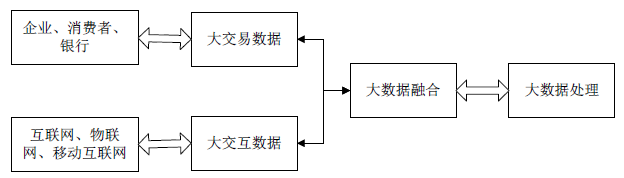
\includegraphics[width=14.0758cm,height=3.9688cm]{assets/diagram.png}
\end{WordParagraph}

% 原文段落 121；图2-1□××××××××××
\begin{WordParagraph}{center}{12}{\WordAutoLine{12}{1.5}}{6}{0}{-6}{0}{0}
\WordAutoSpaceOn
\WordRun{Hei}{Hei}{12}{0}{0}{000000}{0}{图}%
\WordRun{Times}{Song}{12}{0}{0}{000000}{0}{2-1}%
\WordRun{Hei}{Hei}{12}{0}{0}{000000}{0}{□\WordHAnsi{Hei}{×}\hskip0pt plus .05em\relax{}\WordHAnsi{Hei}{×}\hskip0pt plus .05em\relax{}\WordHAnsi{Hei}{×}\hskip0pt plus .05em\relax{}\WordHAnsi{Hei}{×}\hskip0pt plus .05em\relax{}\WordHAnsi{Hei}{×}\hskip0pt plus .05em\relax{}\WordHAnsi{Hei}{×}\hskip0pt plus .05em\relax{}\WordHAnsi{Hei}{×}\hskip0pt plus .05em\relax{}\WordHAnsi{Hei}{×}\hskip0pt plus .05em\relax{}\WordHAnsi{Hei}{×}\hskip0pt plus .05em\relax{}\WordHAnsi{Hei}{×}\hskip0pt plus .05em\relax{}}
\end{WordParagraph}

% 原文段落 122；（图标题：位于图下方，黑体小4号，字母、阿拉伯数字为Time New Roman小4号）
\begin{WordParagraph}{both}{12}{15}{0}{0}{24}{0}{0}
\WordAutoSpaceOn
\WordRun{Kai}{Kai}{12}{0}{0}{FF0000}{0}{（图标题：位于图下方，黑体小4号，字母、阿拉伯数字为Time\WordSpace{1}New\WordSpace{1}Roman小4号）}
\end{WordParagraph}

% 原文段落 123；
\begin{WordParagraph}{both}{12}{\WordAutoLine{12}{1.5}}{0}{0}{24}{0}{0}
\WordAutoSpaceOn
\WordEmpty
\end{WordParagraph}

% 原文段落 124；2.2 UML相关需求分析图（黑体4号加粗,字母、阿拉伯数字为Time New Roman4号加粗）
\begin{WordParagraph}{both}{14}{\WordAutoLine{14}{1.25}}{0}{0}{0}{7.8}{7.8}
\WordAutoSpaceOn
\WordRun{Times}{Song}{14}{1}{0}{000000}{0}{2.2}%
\WordRun{Hei}{Hei}{14}{1}{0}{000000}{0}{\WordSpace{1}UML相关需求分析图}%
\WordRun{Kai}{Kai}{12}{0}{0}{FF0000}{0}{（黑体4号加粗,字母、阿拉伯数字为Time\WordSpace{1}New\WordSpace{1}Roman4号加粗）}
\end{WordParagraph}

% 原文段落 125；选取合适的图表准确说明用户需求，明确所做系统要实现的目标。
\begin{WordParagraph}{both}{12}{\WordAutoLine{12}{1.5}}{0}{0}{24}{0}{0}
\WordAutoSpaceOn
\WordRun{Song}{Song}{12}{0}{0}{000000}{0}{选取合适的图表准确说明用户需求，明确所做系统要实现的目标。}
\end{WordParagraph}

% 原文段落 126；
\begin{WordParagraph}{both}{12}{\WordAutoLine{12}{1.5}}{0}{0}{0}{0}{0}
\WordAutoSpaceOn
\WordEmpty
\end{WordParagraph}

\begin{samepage}

% 原文段落 127；2.3 原型系统设计（黑体4号加粗,字母、阿拉伯数字为Time New Roman4号加粗）
\begin{WordParagraph}{both}{14}{\WordAutoLine{14}{1.25}}{0}{0}{0}{7.8}{7.8}
\WordAutoSpaceOn
\WordRun{Times}{Song}{14}{1}{0}{000000}{0}{2.3}%
\WordRun{Hei}{Hei}{14}{1}{0}{000000}{0}{\WordSpace{1}原型系统设计}%
\WordRun{Kai}{Kai}{12}{0}{0}{FF0000}{0}{（黑体4号加粗,字母、阿拉伯数字为Time\WordSpace{1}New\WordSpace{1}Roman4号加粗）}
\end{WordParagraph}

% 原文段落 128；运用工具设计原型系统，从而更准确说明主要功能和用户交互界面。
\begin{WordParagraph}{both}{12}{\WordAutoLine{12}{1.5}}{0}{0}{24}{0}{0}
\WordAutoSpaceOn
\WordRun{Song}{Song}{12}{0}{0}{000000}{0}{运用工具设计原型系统，从而更准确说明主要功能和用户交互界面。}
\end{WordParagraph}

% 原文段落 129；
\begin{WordParagraph}{both}{12}{\WordAutoLine{12}{1.5}}{0}{0}{0}{0}{0}
\WordAutoSpaceOn
\WordEmpty
\end{WordParagraph}

% 原文段落 130；.......
\begin{WordParagraph}{center}{12}{\WordAutoLine{12}{1.5}}{6}{0}{-6}{0}{0}
\WordAutoSpaceOn
\WordRun{Song}{Song}{12}{0}{0}{000000}{0}{.......}
\end{WordParagraph}

% 原文段落 131；--------章与章之间插入分页符----------
\begin{WordParagraph}{center}{12}{\WordAutoLine{12}{1.5}}{0}{0}{0}{0}{0}
\WordAutoSpaceOn
\WordRun{Times}{Song}{12}{0}{0}{000000}{0}{--------章与章之间插入分页符----------}
\end{WordParagraph}

\end{samepage}

% 原文段落 132；
\newpage
\begin{WordParagraph}{left}{12}{\WordAutoLine{12}{1}}{0}{0}{0}{0}{0}
\WordAutoSpaceOn
\WordEmpty
\end{WordParagraph}

% UTF-8。保留原文文字、颜色、字号、缩进和空段落；最后一项参数是可编辑文本。

% 原文段落 133；3 概要设计和详细设计
\begin{WordParagraph}{center}{18}{\WordAutoLine{18}{1.25}}{0}{0}{0}{7.8}{7.8}
\WordAutoSpaceOn
\WordRun{Times}{Hei}{18}{1}{0}{000000}{0}{3}%
\WordRun{Hei}{Hei}{18}{1}{0}{000000}{0}{\WordSpace{1}}%
\WordRun{Times}{Hei}{18}{1}{0}{000000}{0}{概要设计和详细设计}
\end{WordParagraph}

% 原文段落 134；（黑体小2加粗居中,字母、阿拉伯数字为Time New Roman小2号加粗）
\begin{WordParagraph}{center}{12}{\WordAutoLine{12}{1.25}}{0}{0}{0}{7.8}{7.8}
\WordAutoSpaceOn
\WordRun{Kai}{Kai}{12}{0}{0}{FF0000}{0}{（黑体小2加粗居中}%
\WordRun{Kai}{Kai}{12}{0}{0}{FF0000}{0}{,字母、阿拉伯数字为Time\WordSpace{1}New\WordSpace{1}Roman小2号加粗}%
\WordRun{Kai}{Kai}{12}{0}{0}{FF0000}{0}{）}
\end{WordParagraph}

% 原文段落 135；3.1 系统结构（黑体4号加粗,字母、阿拉伯数字为Time New Roman4号加粗）
\begin{WordParagraph}{both}{14}{\WordAutoLine{14}{1.25}}{0}{0}{0}{7.8}{7.8}
\WordAutoSpaceOn
\WordRun{Times}{Song}{14}{1}{0}{000000}{0}{3.1}%
\WordRun{Hei}{Hei}{14}{1}{0}{000000}{0}{\WordSpace{1}系统结构}%
\WordRun{Kai}{Kai}{12}{0}{0}{FF0000}{0}{（黑体4号加粗,字母、阿拉伯数字为Time\WordSpace{1}New\WordSpace{1}Roman4号加粗）}
\end{WordParagraph}

% 原文段落 136；这部分可根据用户需求，设计和规划一个系统，说明清楚系统应该有哪些功能模块，每个模块做什么。最后给出完整的系统结构图，以及相应的接口设计等。
\begin{WordParagraph}{both}{12}{22.5}{0}{0}{24}{0}{0}
\WordAutoSpaceOff
\WordRun{Song}{Song}{12}{0}{0}{000000}{0}{这部分可根据用户需求，设计和规划一个系统，说明清楚系统应该有哪些功能模块，每个模块做什么。最后给出完整的系统结构图，以及相应的接口设计等。}
\end{WordParagraph}

% 原文段落 137；3.2 类图等（黑体4号加粗,字母、阿拉伯数字为Time New Roman4号加粗）
\begin{WordParagraph}{both}{14}{\WordAutoLine{14}{1.25}}{0}{0}{0}{7.8}{7.8}
\WordAutoSpaceOn
\WordRun{Times}{Song}{14}{1}{0}{000000}{0}{3.2}%
\WordRun{Hei}{Hei}{14}{1}{0}{000000}{0}{\WordSpace{1}类图等}%
\WordRun{Kai}{Kai}{12}{0}{0}{FF0000}{0}{（黑体4号加粗,字母、阿拉伯数字为Time\WordSpace{1}New\WordSpace{1}Roman4号加粗）}
\end{WordParagraph}

% 原文段落 138；运用类图等方法说明系统的设计。
\begin{WordParagraph}{both}{12}{22.5}{0}{0}{24}{0}{0}
\WordAutoSpaceOff
\WordRun{Song}{Song}{12}{0}{0}{000000}{0}{运用类图等方法说明系统的设计。}
\end{WordParagraph}

% 原文段落 139；3.3关键数据结构定义（黑体4号加粗,字母、阿拉伯数字为Time New Roman4号加粗）
\begin{WordParagraph}{both}{14}{\WordAutoLine{14}{1.25}}{0}{0}{0}{7.8}{7.8}
\WordAutoSpaceOn
\WordRun{Times}{Song}{14}{1}{0}{000000}{0}{3.3}%
\WordRun{Hei}{Hei}{14}{1}{0}{000000}{0}{关键数据结构定义}%
\WordRun{Kai}{Kai}{12}{0}{0}{FF0000}{0}{（黑体4号加粗,字母、阿拉伯数字为Time\WordSpace{1}New\WordSpace{1}Roman4号加粗）}
\end{WordParagraph}

% 原文段落 140；这部分要写的：（1）首先描述系统中要处理那些数据，每种类型的数据包括哪些数据项，每个数据项的数据类型；（2) 描述这多种数据在系统中如何关联，可通过图直观的说明这多种数据间的关联。
\begin{WordParagraph}{left}{12}{22.5}{0}{0}{24}{0}{0}
\WordAutoSpaceOff
\WordRun{Song}{Song}{12}{0}{0}{000000}{0}{这部分要写的：（1）首先描述系统中要处理那些数据，每种类型的数据包括哪些数据项，每个数据项的数据类型；（2)\WordSpace{1}描述这多种数据在系统中如何关联，可通过图直观的说明这多种数据间的关联。}
\end{WordParagraph}

% 原文段落 141；3.4 关键算法设计（黑体4号加粗,字母、阿拉伯数字为Time New Roman4号加粗）
\begin{WordParagraph}{both}{14}{\WordAutoLine{14}{1.25}}{0}{0}{0}{7.8}{7.8}
\WordAutoSpaceOn
\WordRun{Times}{Song}{14}{1}{0}{000000}{0}{3.4}%
\WordRun{Hei}{Hei}{14}{1}{0}{000000}{0}{\WordSpace{1}关键算法设计}%
\WordRun{Kai}{Kai}{12}{0}{0}{FF0000}{0}{（黑体4号加粗,字母、阿拉伯数字为Time\WordSpace{1}New\WordSpace{1}Roman4号加粗）}
\end{WordParagraph}

% 原文段落 142；这部分主要描述系统中的模块实现的流程，可采用文字配合流程图的方式表示关键算法的思想及流程。
\begin{WordParagraph}{both}{12}{22.5}{0}{0}{24}{0}{0}
\WordAutoSpaceOff
\WordRun{Times}{Song}{12}{0}{0}{000000}{0}{这部分主要描述系统中的模块实现的流程，可采用文字配合流程图的方式表示关键算法的思想及流程。}
\end{WordParagraph}

% 原文段落 143；3.5 数据管理说明（黑体4号加粗,字母、阿拉伯数字为Time New Roman4号加粗）
\begin{WordParagraph}{both}{14}{\WordAutoLine{14}{1.25}}{0}{0}{0}{7.8}{7.8}
\WordAutoSpaceOn
\WordRun{Times}{Song}{14}{1}{0}{000000}{0}{3.5}%
\WordRun{Hei}{Hei}{14}{1}{0}{000000}{0}{\WordSpace{1}数据管理说明}%
\WordRun{Kai}{Kai}{12}{0}{0}{FF0000}{0}{（黑体4号加粗,字母、阿拉伯数字为Time\WordSpace{1}New\WordSpace{1}Roman4号加粗）}
\end{WordParagraph}

% 原文段落 144；说明整个系统所涉及到的数据用何种方式进行存储和访问。
\begin{WordParagraph}{both}{12}{22.5}{0}{0}{24}{0}{0}
\WordAutoSpaceOff
\WordRun{Times}{Song}{12}{0}{0}{000000}{0}{说明整个系统所涉及到的数据用何种方式进行存储和访问。}
\end{WordParagraph}

% 原文段落 145；
\begin{WordParagraph}{both}{12}{22.5}{0}{0}{24}{0}{0}
\WordAutoSpaceOff
\WordEmpty
\end{WordParagraph}

% 原文段落 146；
\begin{WordParagraph}{both}{12}{22.5}{0}{0}{24}{0}{0}
\WordAutoSpaceOff
\WordEmpty
\end{WordParagraph}

% 原文段落 147；
\begin{WordParagraph}{center}{18}{\WordAutoLine{18}{1.25}}{0}{0}{0}{7.8}{7.8}
\WordAutoSpaceOn
\WordEmpty
\end{WordParagraph}

% 原文段落 148；
\begin{WordParagraph}{center}{18}{\WordAutoLine{18}{1.25}}{0}{0}{0}{7.8}{7.8}
\WordAutoSpaceOn
\WordEmpty
\end{WordParagraph}

% 原文段落 149；
\begin{WordParagraph}{left}{15}{\WordAutoLine{15}{1}}{0}{0}{0}{0}{0}
\WordAutoSpaceOn
\WordEmpty
\end{WordParagraph}

% 原文段落 150；
\begin{WordParagraph}{left}{15}{\WordAutoLine{15}{1}}{0}{0}{0}{0}{0}
\WordAutoSpaceOn
\WordEmpty
\end{WordParagraph}

% UTF-8。保留原文文字、颜色、字号、缩进和空段落；最后一项参数是可编辑文本。

% 原文段落 151；4 实现与测试
\begin{WordParagraph}{center}{18}{\WordAutoLine{18}{1.25}}{0}{0}{0}{7.8}{7.8}
\WordAutoSpaceOn
\WordRun{Times}{Hei}{18}{1}{0}{000000}{0}{4}%
\WordRun{Hei}{Hei}{18}{1}{0}{000000}{0}{\WordSpace{1}}%
\WordRun{Times}{Hei}{18}{1}{0}{000000}{0}{实现与测试}
\end{WordParagraph}

% 原文段落 152；（黑体小2加粗居中,字母、阿拉伯数字为Time New Roman小2号加粗）
\begin{WordParagraph}{center}{12}{\WordAutoLine{12}{1.25}}{0}{0}{0}{7.8}{7.8}
\WordAutoSpaceOn
\WordRun{Kai}{Kai}{12}{0}{0}{FF0000}{0}{（黑体小2加粗居中}%
\WordRun{Kai}{Kai}{12}{0}{0}{FF0000}{0}{,字母、阿拉伯数字为Time\WordSpace{1}New\WordSpace{1}Roman小2号加粗}%
\WordRun{Kai}{Kai}{12}{0}{0}{FF0000}{0}{）}
\end{WordParagraph}

% 原文段落 153；4.1实现环境与代码管理（黑体4号加粗,字母、阿拉伯数字为Time New Roman4号加粗）
\begin{WordParagraph}{both}{14}{\WordAutoLine{14}{1.25}}{0}{0}{0}{7.8}{7.8}
\WordAutoSpaceOn
\WordRun{Times}{Song}{14}{1}{0}{000000}{0}{4.1}%
\WordRun{Hei}{Hei}{14}{1}{0}{000000}{0}{实现环境与代码管理}%
\WordRun{Kai}{Kai}{12}{0}{0}{FF0000}{0}{（黑体4号加粗,字母、阿拉伯数字为Time\WordSpace{1}New\WordSpace{1}Roman4号加粗）}
\end{WordParagraph}

% 原文段落 154；这部分可首先叙述所设计软件实现的软硬件环境，代码版本管理的签入记录需截图进行说明。例如使用码云平台签入记录截图如图4-1所示（也可使用其他工具）：
\begin{WordParagraph}{both}{12}{22.5}{0}{0}{24}{0}{0}
\WordAutoSpaceOff
\WordRun{Song}{Song}{12}{0}{0}{000000}{0}{这部分可首先叙述所设计软件实现的软硬件环境，代码版本管理的签入记录需截图进行说明。例如使用码云平台签入记录截图如图}%
\WordRun{Times}{Song}{12}{0}{0}{000000}{0}{4-1}%
\WordRun{Song}{Song}{12}{0}{0}{000000}{0}{所示（也可使用其他工具）：}
\end{WordParagraph}

% 原文段落 155；
\begin{WordParagraph}{both}{12}{\WordAutoLine{12}{1}}{0}{0}{24}{0}{0}
\WordAutoSpaceOff
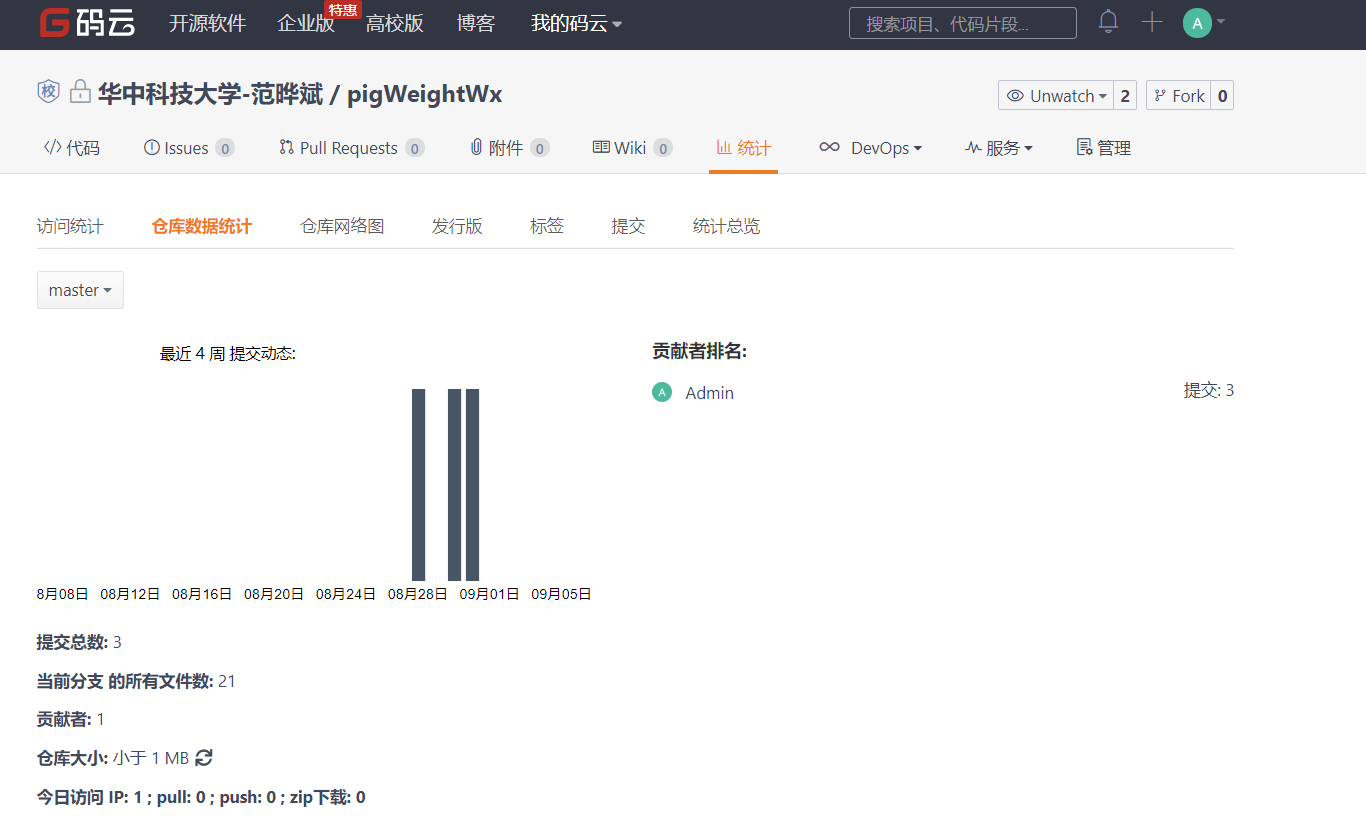
\includegraphics[width=12.4672cm,height=7.657cm]{assets/gitee-example.png}
\end{WordParagraph}

% 原文段落 156；图4-1 码云平台代码签入示例
\begin{WordParagraph}{center}{12}{\WordAutoLine{12}{1}}{0}{0}{24}{0}{0}
\WordAutoSpaceOff
\WordRun{Song}{Song}{12}{0}{0}{000000}{0}{图}%
\WordRun{Times}{Song}{12}{0}{0}{000000}{0}{4-1}%
\WordRun{Song}{Song}{12}{0}{0}{000000}{0}{\WordSpace{1}码云平台代码签入示例}
\end{WordParagraph}

% 原文段落 157；4.2 关键函数说明（黑体4号加粗,字母、阿拉伯数字为Time New Roman4号加粗）
\begin{WordParagraph}{both}{14}{\WordAutoLine{14}{1.25}}{0}{0}{0}{7.8}{7.8}
\WordAutoSpaceOn
\WordRun{Times}{Song}{14}{1}{0}{000000}{0}{4.2}%
\WordRun{Hei}{Hei}{14}{1}{0}{000000}{0}{\WordSpace{1}关键函数说明}%
\WordRun{Kai}{Kai}{12}{0}{0}{FF0000}{0}{（黑体4号加粗,字母、阿拉伯数字为Time\WordSpace{1}New\WordSpace{1}Roman4号加粗）}
\end{WordParagraph}

% 原文段落 158；程序代码部分在这里不需要给出来，只需要叙述清楚在系统中包括哪些函数，各函数的说明，如何利用这些函数实现系统各模块的功能，以及函数间的调用关系（可用图表示出来）。程序详见附录。
\begin{WordParagraph}{both}{12}{\WordAutoLine{12}{1.5}}{0}{0}{24}{0}{0}
\WordAutoSpaceOn
\WordRun{Song}{Song}{12}{0}{0}{000000}{0}{程序代码部分在这里不需要给出来，只需要叙述清楚在系统中包括哪些函数，各函数的说明，如何利用这些函数实现系统各模块的功能，以及函数间的调用关系（可用图表示出来）。程序详见附录。}
\end{WordParagraph}

% 原文段落 159；4.3 测试计划和测试用例（黑体4号加粗,字母、阿拉伯数字为Time New Roman4号加粗）
\begin{WordParagraph}{both}{14}{\WordAutoLine{14}{1.25}}{0}{0}{0}{7.8}{7.8}
\WordAutoSpaceOn
\WordRun{Times}{Song}{14}{1}{0}{000000}{0}{4.3}%
\WordRun{Hei}{Hei}{14}{1}{0}{000000}{0}{\WordSpace{1}测试计划和测试用例}%
\WordRun{Kai}{Kai}{12}{0}{0}{FF0000}{0}{（黑体4号加粗,字母、阿拉伯数字为Time\WordSpace{1}New\WordSpace{1}Roman4号加粗）}
\end{WordParagraph}

% 原文段落 160；首先叙述一下常用的软件测试方法，在选择几个主要的功能模块（自行掌握数量，关键要体现你的水平的一些模块）描述测试过程，（1）先明确模块的功能、设计目标等。（2）分析、叙述如何选取测试数据，要求有完整的测
\begin{WordParagraph}{both}{12}{22.5}{0}{0}{24}{0}{0}
\WordAutoSpaceOff
\WordRun{Song}{Song}{12}{0}{0}{000000}{0}{首先叙述一下常用的软件测试方法，在选择几个主要的功能模块（自行掌握数量，关键要体现你的水平的一些模块）描述测试过程，（1）先明确模块的功能、设计目标等。（2）分析、叙述如何选取测试数据，要求有完整的测试计划和测试用例，说明测试运行结果（这时可用截图）。}
\end{WordParagraph}

% 原文段落 161；4.4 结果分析（黑体4号加粗,字母、阿拉伯数字为Time New Roman4号加粗）
\begin{WordParagraph}{both}{14}{\WordAutoLine{14}{1.25}}{0}{0}{0}{7.8}{7.8}
\WordAutoSpaceOn
\WordRun{Times}{Song}{14}{1}{0}{000000}{0}{4.4}%
\WordRun{Hei}{Hei}{14}{1}{0}{000000}{0}{\WordSpace{1}结果分析}%
\WordRun{Kai}{Kai}{12}{0}{0}{FF0000}{0}{（黑体4号加粗,字母、阿拉伯数字为Time\WordSpace{1}New\WordSpace{1}Roman4号加粗）}
\end{WordParagraph}

% 原文段落 162；根据测试分析运行结果、确认软件是否满足需求。
\begin{WordParagraph}{both}{12}{\WordAutoLine{12}{1.25}}{0}{0}{24}{7.8}{7.8}
\WordAutoSpaceOn
\WordRun{Song}{Song}{12}{0}{0}{000000}{0}{根据测试分析运行结果、确认软件是否满足需求。}
\end{WordParagraph}

% 原文段落 163；
\newpage
\begin{WordParagraph}{left}{12}{\WordAutoLine{12}{1}}{0}{0}{0}{0}{0}
\WordAutoSpaceOn
\WordEmpty
\end{WordParagraph}

% UTF-8。保留原文文字、颜色、字号、缩进和空段落；最后一项参数是可编辑文本。

% 原文段落 164；5 总结
\begin{WordParagraph}{center}{18}{\WordAutoLine{18}{1.25}}{0}{0}{0}{7.8}{7.8}
\WordAutoSpaceOn
\WordRun{Times}{Hei}{18}{1}{0}{000000}{0}{5}%
\WordRun{Hei}{Hei}{18}{1}{0}{000000}{0}{\WordSpace{1}总结}
\end{WordParagraph}

% 原文段落 165；（黑体小2加粗居中,字母、阿拉伯数字为Time New Roman小2号加粗）
\begin{WordParagraph}{center}{12}{\WordAutoLine{12}{1.25}}{0}{0}{0}{7.8}{7.8}
\WordAutoSpaceOn
\WordRun{Kai}{Kai}{12}{0}{0}{FF0000}{0}{（黑体小2加粗居中}%
\WordRun{Kai}{Kai}{12}{0}{0}{FF0000}{0}{,字母、阿拉伯数字为Time\WordSpace{1}New\WordSpace{1}Roman小2号加粗}%
\WordRun{Kai}{Kai}{12}{0}{0}{FF0000}{0}{）}
\end{WordParagraph}

% 原文段落 166；5.1 用户反馈（黑体4号加粗,字母、阿拉伯数字为Time New Roman4号加粗）
\begin{WordParagraph}{both}{14}{\WordAutoLine{14}{1.25}}{0}{0}{0}{7.8}{7.8}
\WordAutoSpaceOn
\WordRun{Times}{Song}{14}{1}{0}{000000}{0}{5.1}%
\WordRun{Hei}{Hei}{14}{1}{0}{000000}{0}{\WordSpace{1}用户反馈}%
\WordRun{Kai}{Kai}{12}{0}{0}{FF0000}{0}{（黑体4号加粗,字母、阿拉伯数字为Time\WordSpace{1}New\WordSpace{1}Roman4号加粗）}
\end{WordParagraph}

% 原文段落 167；包括用户的使用记录，照片，视频等。
\begin{WordParagraph}{both}{12}{22.5}{0}{0}{24}{0}{0}
\WordAutoSpaceOn
\WordRun{Times}{Song}{12}{0}{0}{000000}{0}{包括用户的使用记录，照片，视频等}%
\WordRun{Song}{Song}{12}{0}{0}{000000}{0}{。}
\end{WordParagraph}

% 原文段落 168；
\begin{WordParagraph}{both}{12}{\WordAutoLine{12}{1.5}}{0}{0}{24}{0}{0}
\WordAutoSpaceOn
\WordEmpty
\end{WordParagraph}

% 原文段落 169；5.1 全文总结（黑体4号加粗,字母、阿拉伯数字为Time New Roman4号加粗）
\begin{WordParagraph}{both}{14}{\WordAutoLine{14}{1.25}}{0}{0}{0}{7.8}{7.8}
\WordAutoSpaceOn
\WordRun{Times}{Song}{14}{1}{0}{000000}{0}{5.1\WordSpace{1}}%
\WordRun{Hei}{Hei}{14}{1}{0}{000000}{0}{全文总结}%
\WordRun{Kai}{Kai}{12}{0}{0}{FF0000}{0}{（黑体4号加粗,字母、阿拉伯数字为Time\WordSpace{1}New\WordSpace{1}Roman4号加粗）}
\end{WordParagraph}

% 原文段落 170；对自己的工作做个总结，主要工作如下：
\begin{WordParagraph}{both}{12}{22.5}{0}{0}{24}{0}{0}
\WordAutoSpaceOn
\WordRun{Song}{Song}{12}{0}{0}{000000}{0}{对自己的工作做个总结，主要工作如下：}
\end{WordParagraph}

% 原文段落 171；（1）对XXXXX。
\begin{WordParagraph}{both}{12}{22.5}{0}{0}{24}{0}{0}
\WordAutoSpaceOn
\WordRun{Song}{Song}{12}{0}{0}{000000}{0}{（1）对XXXXX。}
\end{WordParagraph}

% 原文段落 172；（2）
\begin{WordParagraph}{both}{12}{22.5}{0}{0}{24}{0}{0}
\WordAutoSpaceOn
\WordRun{Song}{Song}{12}{0}{0}{000000}{0}{（2）}
\end{WordParagraph}

% 原文段落 173；（3）
\begin{WordParagraph}{both}{12}{22.5}{0}{0}{24}{0}{0}
\WordAutoSpaceOn
\WordRun{Song}{Song}{12}{0}{0}{000000}{0}{（3）}
\end{WordParagraph}

% 原文段落 174；
\begin{WordParagraph}{both}{12}{22.5}{0}{0}{24}{0}{0}
\WordAutoSpaceOff
\WordEmpty
\end{WordParagraph}

% 原文段落 175；
\begin{WordParagraph}{left}{12}{\WordAutoLine{12}{1}}{0}{0}{0}{0}{0}
\WordAutoSpaceOn
\WordEmpty
\end{WordParagraph}

% 原文段落 176；
\begin{WordParagraph}{both}{12}{22.5}{0}{0}{24}{0}{0}
\WordAutoSpaceOff
\WordEmpty
\end{WordParagraph}

% 原文段落 177；
\newpage
\begin{WordParagraph}{both}{12}{\WordAutoLine{12}{1.25}}{0}{0}{0}{0}{0}
\WordAutoSpaceOn
\WordEmpty
\end{WordParagraph}

% UTF-8。保留原文文字、颜色、字号、缩进和空段落；最后一项参数是可编辑文本。

% 原文段落 178；6 体会(黑体小2号加粗居中)
\begin{WordParagraph}{center}{18}{\WordAutoLine{18}{1.25}}{0}{0}{0}{7.8}{7.8}
\WordAutoSpaceOn
\WordRun{Times}{Hei}{18}{1}{0}{000000}{0}{6\WordSpace{1}体会}%
\WordRun{Kai}{Kai}{12}{0}{0}{FF0000}{0}{(黑体小2号加粗居中)}
\end{WordParagraph}

% 原文段落 179；这部分需要每个组员分别就自己的分工进行撰写，重点描述在软件开发中遇到的挫折与如何解决的方法，不要写套话。
\begin{WordParagraph}{both}{12}{\WordAutoLine{12}{1.35}}{0}{0}{24}{0}{0}
\WordAutoSpaceOn
\WordRun{Song}{Song}{12}{0}{0}{000000}{0}{这部分需要每个组员分别就自己的分工进行撰写，重点描述在软件开发中遇到的挫折与如何解决的方法，不要写套话。}
\end{WordParagraph}

% 原文段落 180；XX同学，分工：XXX，体会：XXXXX
\begin{WordParagraph}{both}{12}{\WordAutoLine{12}{1.35}}{0}{0}{24}{0}{0}
\WordAutoSpaceOn
\WordRun{Song}{Song}{12}{0}{0}{000000}{0}{XX同学，分工：XXX，体会：XXXXX}
\end{WordParagraph}

% 原文段落 181；
\begin{WordParagraph}{both}{12}{\WordAutoLine{12}{1.35}}{0}{0}{24}{0}{0}
\WordAutoSpaceOn
\WordEmpty
\end{WordParagraph}

% 原文段落 182；
\begin{WordParagraph}{left}{12}{\WordAutoLine{12}{1}}{0}{0}{0}{0}{0}
\WordAutoSpaceOn
\WordEmpty
\end{WordParagraph}

% 原文段落 183；
\newpage
\begin{WordParagraph}{left}{12}{\WordAutoLine{12}{1}}{0}{0}{0}{0}{0}
\WordAutoSpaceOn
\WordEmpty
\end{WordParagraph}

% UTF-8。保留原文文字、颜色、字号、缩进和空段落；最后一项参数是可编辑文本。

% 原文段落 184；附录 (黑体小2号加粗居中)
\begin{WordParagraph}{center}{18}{\WordAutoLine{18}{1.25}}{0}{0}{0}{7.8}{7.8}
\WordAutoSpaceOn
\WordRun{Hei}{Hei}{18}{1}{0}{000000}{0}{附录\WordSpace{1}}%
\WordRun{Kai}{Kai}{12}{0}{0}{FF0000}{0}{(黑体小2号加粗居中)}
\end{WordParagraph}

% 原文段落 185；关键的源代码等。
\begin{WordParagraph}{both}{12}{\WordAutoLine{12}{1.5}}{0}{0}{24}{0}{0}
\WordAutoSpaceOn
\WordRun{Song}{Song}{12}{0}{0}{000000}{0}{关键的源代码等。}
\end{WordParagraph}

% 原文段落 186；( 宋体5号，英文Times new roman字体)
\begin{WordParagraph}{both}{12}{\WordAutoLine{12}{1.5}}{0}{0}{0}{0}{0}
\WordAutoSpaceOn
\WordRun{Kai}{Kai}{12}{0}{0}{FF0000}{0}{(\WordSpace{1}宋体5号，英文Times\WordSpace{1}new\WordSpace{1}roman字体)}
\end{WordParagraph}

% 原文段落 187；……
\begin{WordParagraph}{center}{12}{\WordAutoLine{12}{1.5}}{0}{0}{0}{0}{0}
\WordAutoSpaceOn
\WordRun{Song}{Song}{12}{0}{0}{000000}{0}{……}
\end{WordParagraph}

% 原文段落 188；……
\begin{WordParagraph}{center}{12}{\WordAutoLine{12}{1.5}}{0}{0}{0}{0}{0}
\WordAutoSpaceOn
\WordRun{Song}{Song}{12}{0}{0}{000000}{0}{……}
\end{WordParagraph}

% 原文段落 189；……
\begin{WordParagraph}{center}{12}{\WordAutoLine{12}{1.5}}{0}{0}{0}{0}{0}
\WordAutoSpaceOn
\WordRun{Song}{Song}{12}{0}{0}{000000}{0}{……}
\end{WordParagraph}

% 原文段落 190；
\begin{WordParagraph}{center}{12}{\WordAutoLine{12}{1.25}}{0}{0}{0}{0}{0}
\WordAutoSpaceOn
\WordEmpty
\end{WordParagraph}

% 原文段落 191；
\begin{WordParagraph}{both}{12}{23}{0}{0}{24}{0}{0}
\WordAutoSpaceOn
\WordEmpty
\end{WordParagraph}

% 原文段落 192；
\begin{WordParagraph}{center}{12}{\WordAutoLine{12}{1.5}}{0}{0}{0}{0}{0}
\WordAutoSpaceOn
\WordEmpty
\end{WordParagraph}

% 原文段落 193；
\begin{WordParagraph}{center}{12}{\WordAutoLine{12}{1.5}}{0}{0}{0}{0}{0}
\WordAutoSpaceOn
\WordEmpty
\end{WordParagraph}

% 原文段落 194；
\begin{WordParagraph}{center}{12}{\WordAutoLine{12}{1.5}}{0}{0}{0}{0}{0}
\WordAutoSpaceOn
\WordEmpty
\end{WordParagraph}

% 原文段落 195；
\begin{WordParagraph}{center}{12}{\WordAutoLine{12}{1.5}}{0}{0}{0}{0}{0}
\WordAutoSpaceOn
\WordEmpty
\end{WordParagraph}

% 原文段落 196；
\begin{WordParagraph}{center}{12}{\WordAutoLine{12}{1.5}}{0}{0}{0}{0}{0}
\WordAutoSpaceOn
\WordEmpty
\end{WordParagraph}

% 原文段落 197；
\begin{WordParagraph}{center}{12}{\WordAutoLine{12}{1.5}}{0}{0}{0}{0}{0}
\WordAutoSpaceOn
\WordEmpty
\end{WordParagraph}

% 原文段落 198；
\begin{WordParagraph}{center}{12}{\WordAutoLine{12}{1.5}}{0}{0}{0}{0}{0}
\WordAutoSpaceOn
\WordEmpty
\end{WordParagraph}

% 原文段落 199；
\begin{WordParagraph}{center}{12}{\WordAutoLine{12}{1.5}}{0}{0}{0}{0}{0}
\WordAutoSpaceOn
\WordEmpty
\end{WordParagraph}

% 原文段落 200；
\begin{WordParagraph}{both}{12}{\WordAutoLine{12}{1.25}}{0}{0}{0}{0}{0}
\WordAutoSpaceOn
\WordEmpty
\end{WordParagraph}

% 原文段落 201；
\begin{WordParagraph}{both}{12}{\WordAutoLine{12}{1.25}}{0}{0}{0}{0}{0}
\WordAutoSpaceOn
\WordEmpty
\end{WordParagraph}

% 原文段落 202；
\begin{WordParagraph}{both}{12}{\WordAutoLine{12}{1.25}}{0}{0}{0}{0}{0}
\WordAutoSpaceOn
\WordEmpty
\end{WordParagraph}

% 原文段落 203；
\begin{WordParagraph}{both}{12}{\WordAutoLine{12}{1.25}}{0}{0}{0}{0}{0}
\WordAutoSpaceOn
\WordEmpty
\end{WordParagraph}

% 原文段落 204；
\begin{WordParagraph}{both}{12}{\WordAutoLine{12}{1.25}}{0}{0}{0}{0}{0}
\WordAutoSpaceOn
\WordEmpty
\end{WordParagraph}

% 原文段落 205；
\begin{WordParagraph}{both}{12}{\WordAutoLine{12}{1.25}}{0}{0}{0}{0}{0}
\WordAutoSpaceOn
\WordEmpty
\end{WordParagraph}

% 原文段落 206；
\begin{WordParagraph}{both}{12}{\WordAutoLine{12}{1.25}}{0}{0}{0}{0}{0}
\WordAutoSpaceOn
\WordEmpty
\end{WordParagraph}

% 原文段落 207；
\begin{WordParagraph}{both}{12}{\WordAutoLine{12}{1.25}}{0}{0}{0}{0}{0}
\WordAutoSpaceOn
\WordEmpty
\end{WordParagraph}

% 原文段落 208；
\begin{WordParagraph}{both}{12}{\WordAutoLine{12}{1.25}}{0}{0}{0}{0}{0}
\WordAutoSpaceOn
\WordEmpty
\end{WordParagraph}

% 原文段落 209；
\begin{WordParagraph}{both}{12}{\WordAutoLine{12}{1.25}}{0}{0}{0}{0}{0}
\WordAutoSpaceOn
\WordEmpty
\end{WordParagraph}

% 原文段落 210；
\begin{WordParagraph}{both}{12}{\WordAutoLine{12}{1.25}}{0}{0}{0}{0}{0}
\WordAutoSpaceOn
\WordEmpty
\end{WordParagraph}

% 原文段落 211；
\begin{WordParagraph}{both}{12}{\WordAutoLine{12}{1.25}}{0}{0}{0}{0}{0}
\WordAutoSpaceOn
\WordEmpty
\end{WordParagraph}

% 原文段落 212；
\begin{WordParagraph}{both}{12}{\WordAutoLine{12}{1.25}}{0}{0}{0}{0}{0}
\WordAutoSpaceOn
\WordEmpty
\end{WordParagraph}

% 原文段落 213；
\begin{WordParagraph}{both}{12}{\WordAutoLine{12}{1.25}}{0}{0}{0}{0}{0}
\WordAutoSpaceOn
\WordEmpty
\end{WordParagraph}

% 原文段落 214；
\begin{WordParagraph}{both}{12}{\WordAutoLine{12}{1.25}}{0}{0}{0}{0}{0}
\WordAutoSpaceOn
\WordEmpty
\end{WordParagraph}

% 原文段落 215；
\begin{WordParagraph}{center}{15}{\WordAutoLine{15}{1}}{0}{0}{0}{24}{12}
\WordAutoSpaceOn
\WordEmpty
\end{WordParagraph}

\end{document}
